%\documentclass[11pt,leqno]{article}
\documentclass[11pt]{amsart}
\usepackage{comment}
%auto-ignore
%!TEX root = webs.tex
%this ensures the arxiv doesn't try to start TeXing here.

\usepackage{amsmath,amssymb,amsfonts,amsthm}
\usepackage{ifpdf}

\usepackage{comment}

\usepackage[all]{xy}
\SelectTips{cm}{}
% This may speed up compilation of complex documents with many xymatrices.
%\CompileMatrices

\usepackage[section]{placeins}
\usepackage{leftidx}
\usepackage{stmaryrd} % additional math symbols, e.g. \mapsfrom
%\usepackage{libertine}
%\usepackage[T1]{fontenc}
\usepackage{microtype}

% ----------------------------------------------------------------
\vfuzz5pt % Don't report over-full v-boxes if over-edge is small
\hfuzz5pt % Don't report over-full h-boxes if over-edge is small
% ----------------------------------------------------------------

% don't warn about PDF 1.5 (default was 1.4); dangerous?
\pdfminorversion=5

% diagrams -------------------------------------------------------
% figures ---------------------------------------------------------
\newcommand{\pathtotrunk}{./}
\newcommand{\pathtodiagrams}{\pathtotrunk}

\newcommand{\mathfig}[2]{\ensuremath{\hspace{-3pt}\begin{array}{c}%
  \raisebox{-2.5pt}{\includegraphics[width=#1\textwidth]{\pathtodiagrams #2}}%
\end{array}\hspace{-3pt}}}
\newcommand{\reflectmathfig}[2]{{\hspace{-3pt}\begin{array}{c}%
  \raisebox{-2.5pt}{\reflectbox{\includegraphics[width=#1\textwidth]{\pathtodiagrams #2}}}%
\end{array}\hspace{-3pt}}}
\newcommand{\rotatemathfig}[3]{{\hspace{-3pt}\begin{array}{c}%
  \raisebox{-2.5pt}{\rotatebox{#2}{\includegraphics[height=#1\textwidth]{\pathtodiagrams #3}}}%
\end{array}\hspace{-3pt}}}
\newcommand{\placefig}[2]{\includegraphics[width=#1\linewidth]{\pathtodiagrams #2}}

\newcommand{\arxiv}[1]{\href{http://arxiv.org/abs/#1}{\tt arXiv:\nolinkurl{#1}}}
\newcommand{\doi}[1]{\href{http://dx.doi.org/#1}{{\tt DOI:#1}}}
\newcommand{\euclid}[1]{\href{http://projecteuclid.org/euclid.cmp/#1}{{\tt #1}}}
\newcommand{\mathscinet}[1]{\href{http://www.ams.org/mathscinet-getitem?mr=#1}{\tt #1}}
\newcommand{\googlebooks}[1]{(preview at \href{http://books.google.com/books?id=#1}{google books})}


% THEOREMS -------------------------------------------------------
\theoremstyle{plain}
%\newtheorem*{fact}{Fact}
\newtheorem{prop}{Proposition}[subsection]
\makeatletter
\@addtoreset{prop}{section}
\makeatother
\newtheorem{conj}[prop]{Conjecture}
\newtheorem{thm}[prop]{Theorem}
\newtheorem{lem}[prop]{Lemma}
\newtheorem*{lem*}{Lemma}
\newtheorem{cor}[prop]{Corollary}
\newtheorem*{cor*}{Corollary}
\newtheorem*{exc}{Exercise}
\newtheorem{defn}[prop]{Definition}         % numbered definition
\newtheorem*{defn*}{Definition}             % unnumbered definition
\newtheorem{question}{Question}
\newtheorem{property}[prop]{Property}
\newenvironment{rem}{\vspace{0.3cm}\noindent\textsl{Remark.}}{}  % perhaps looks better than rem above?
\newenvironment{example}{\vspace{0.3cm}\noindent\textbf{Example.}}{}  % perhaps looks better than rem above?
\newtheorem{rem*}[prop]{Remark}
\numberwithin{equation}{section}
%% example, claim and remark are defined in article_preamble.tex, for compatibility with beamer and PNAS


% Marginal notes in draft mode -----------------------------------
\newcounter{comment}
\newcommand{\noop}[1]{}
\newcommand{\todo}[1]{\textbf{\color[rgb]{.8,.2,.5}\small TODO: #1}}

% \mathrlap -- a horizontal \smash--------------------------------
% For comparison, the existing overlap macros:
% \def\llap#1{\hbox to 0pt{\hss#1}}
% \def\rlap#1{\hbox to 0pt{#1\hss}}
\def\clap#1{\hbox to 0pt{\hss#1\hss}}
\def\mathllap{\mathpalette\mathllapinternal}
\def\mathrlap{\mathpalette\mathrlapinternal}
\def\mathclap{\mathpalette\mathclapinternal}
\def\mathllapinternal#1#2{%
\llap{$\mathsurround=0pt#1{#2}$}}
\def\mathrlapinternal#1#2{%
\rlap{$\mathsurround=0pt#1{#2}$}}
\def\mathclapinternal#1#2{%
\clap{$\mathsurround=0pt#1{#2}$}}

% MATH -----------------------------------------------------------
\newcommand{\id}{\boldsymbol{1}}
\renewcommand{\imath}{\mathfrak{i}}
\renewcommand{\jmath}{\mathfrak{j}}

\newcommand{\ssum}[1]{\Sigma#1}
\newcommand{\sumhat}{\overline{\sum}}
\newcommand{\sumtah}{\underline{\sum}}

\newcommand{\lmod}[1]{\leftidx{_{#1}}{\operatorname{mod}}{}}

\newcommand{\into}{\hookrightarrow}
\newcommand{\onto}{\twoheadrightarrow}
\newcommand{\iso}{\cong}
\newcommand{\quism}{\underset{\text{q.i.}}{\simeq}}
\newcommand{\htpy}{\simeq}
\newcommand{\actsOn}{\circlearrowright}
\newcommand{\xto}[1]{\xrightarrow{#1}}
\newcommand{\isoto}{\xto{\iso}}
\newcommand{\quismto}{\xrightarrow[\text{q.i.}]{\iso}}
\newcommand{\diffeoto}{\xrightarrow[\text{diffeo}]{\iso}}
\newcommand{\htpyto}{\xrightarrow[\text{htpy}]{\htpy}}

\newcommand{\restrict}[2]{#1{}_{\mid #2}{}}
\newcommand{\set}[1]{\left\{#1\right\}}
\newcommand{\setc}[2]{\setcl{#1}{#2}}
\newcommand{\setcl}[2]{\left\{ \left. #1 \;\right| \; #2 \right\}}
\newcommand{\setcr}[2]{\left\{ #1 \;\left| \; #2 \right\}\right.}

\newcommand{\floor}[1]{\left\lfloor#1\right\rfloor}
\newcommand{\norm}[1]{\left|\left|#1\right|\right|}
\newcommand{\abs}[1]{\left|#1\right|}

\newcommand{\qi}[2][q]{\left[#2\right]_{#1}}
\newcommand{\qBinomial}[3][q]{\genfrac{[}{]}{0pt}{}{#2}{#3}_{#1}}
\newcommand{\qPoch}[3]{\left(#1;#2\right)_{#3}}

\newcommand{\card}[1]{\sharp{#1}}

\newcommand{\bdy}{\partial}
\newcommand{\compose}{\circ}
\newcommand{\eset}{\emptyset}

\newcommand{\directSum}{\oplus}
\newcommand{\DirectSum}{\bigoplus}
\newcommand{\tensor}{\otimes}
\newcommand{\Tensor}{\bigotimes}

\newcommand{\Homa}[3]{\Hom_{#1}\left(#2,#3\right)}
\newcommand{\Hom}{\operatorname{Hom}}
\newcommand{\End}[1]{\operatorname{End}\left(#1\right)}

% ----------------------------------------------------------------

\ifpdf
	\usepackage[pdftex,plainpages=false,hypertexnames=false,pdfpagelabels]{hyperref}
	\usepackage[pdftex]{graphicx}
\else
	\usepackage[plainpages=false,hypertexnames=false,pdfpagelabels]{hyperref}
	\usepackage{graphicx}
\fi

%must load tikz after graphicx
\usepackage{tikz}
\usetikzlibrary{shapes}
\usetikzlibrary{backgrounds}
\usetikzlibrary{decorations,decorations.pathreplacing,decorations.markings}
\usetikzlibrary{fit,calc,through}
\usetikzlibrary{external}

\tikzstyle{mid>}=[decoration={markings, mark=at position 0.5 with {\arrow{>}}}, postaction={decorate}]
\tikzstyle{mid<}=[decoration={markings, mark=at position 0.5 with {\arrow{<}}}, postaction={decorate}]
\tikzstyle{upper>}=[decoration={markings, mark=at position 0.8 with {\arrow{>}}}, postaction={decorate}]
\tikzstyle{upper<}=[decoration={markings, mark=at position 0.8 with {\arrow{<}}}, postaction={decorate}]
\tikzstyle{lower>}=[decoration={markings, mark=at position 0.2 with {\arrow{>}}}, postaction={decorate}]
\tikzstyle{lower<}=[decoration={markings, mark=at position 0.2 with {\arrow{<}}}, postaction={decorate}]

\def\Foam{{\mathcal{F}{\rm oam}}}
\newcommand{\alt}{\wedge}
\newcommand{\Alt}[2]{{\textstyle\bigwedge^{#1}_{#2}}}
\newcommand{\Usl}[1]{U\sl_{#1}}
\newcommand{\one}{1}
\def\sA{\mathcal{A}}
\def\l{\lambda}
\def\bZ{{\mathbb{Z}}}
\def\sl{{\mathfrak{sl}}}
\def\Sp{{\mathcal{S}p}}
\def\FSp{{\mathcal{FS}p}}
\def\bC{{\mathbb{C}}}
\def\g{{\mathfrak{g}}}
\def\SL{{\rm{SL}}}
\def\GL{{\rm{GL}}}
\def\gl{{\mathfrak{gl}}}
\def\dU{\dot{{\mathcal{U}}}_q}
\def\Uq{\mathcal{U}_q}
\def\Rep{\mathcal{R}ep}
\def\la{\langle}
\def\ra{\rangle}
\def\dalg{\dot{{U}}_q}

\newcommand{\ul}[1]{{\underline{#1}}}

%\newcommand{\RepSL}[1]{\mathcal{R}ep(SL_{#1})}
\newcommand{\Lad}{\mathcal{L}ad}

\usepackage{environ}
\usepackage{xargs}

\newcommandx{\NewEnvironx}[5][2,3]{%
  \expandafter\newcommandx\csname start#1\endcsname[#2][#3]{#4}%
  \NewEnviron{#1}{\csname start#1\expandafter\endcsname\BODY #5}}

\newcommand{\ladderX}{1.5}
\newcommand{\ladderY}{1.5}
\newcommand{\ladderR}{0.6}
\newcommand{\laddercoordinates}[2]{
\foreach \x in {0,...,#1} {
	\foreach \y in {0,...,#2} {
		\coordinate (l\x\y) at (\x * \ladderX, \y * \ladderY);
		\coordinate (u\x\y) at ($(l\x\y)+\ladderR*(0,\ladderY)$);
		\coordinate (d\x\y) at ($(l\x\y)+(0,\ladderY)-\ladderR*(0,\ladderY)$);
	}
}
}
\newcommand{\ladderEn}[5]{
\draw[mid>] (l#1#2) -- (d#1#2);
\draw[mid>] (d#1#2) -- ($(l#1#2)+(0,\ladderY)$) node[left] {#3};
\draw[mid>] ($(l#1#2)+(\ladderX,0)$) -- ($(u#1#2)+(\ladderX,0)$);
\draw[mid>] ($(u#1#2)+(\ladderX,0)$) -- ($(l#1#2)+(\ladderX,\ladderY)$) node[right] {#4};
\draw[mid>] (d#1#2) --node[above]{#5} ($(u#1#2)+(\ladderX,0)$);
}
\newcommand{\ladderE}[4]{\ladderEn{#1}{#2}{#3}{#4}{}}
\newcommand{\ladderFn}[5]{
\draw[mid>] (l#1#2) -- (u#1#2);
\draw[mid>] (u#1#2) -- ($(l#1#2)+(0,\ladderY)$) node[left] {#3};
\draw[mid>] ($(l#1#2)+(\ladderX,0)$) -- ($(d#1#2)+(\ladderX,0)$);
\draw[mid>] ($(d#1#2)+(\ladderX,0)$) -- ($(l#1#2)+(\ladderX,\ladderY)$) node[right] {#4};
\draw[mid>] ($(d#1#2)+(\ladderX,0)$) --node[above]{#5} (u#1#2);
}
\newcommand{\ladderF}[4]{\ladderFn{#1}{#2}{#3}{#4}{}}
\newcommand{\ladderIn}[3]{\draw[mid>] (l#1#2) -- +($#3*(0,\ladderY)$);}
\newcommand{\ladderI}[2]{\ladderIn{#1}{#2}{1}}

\NewEnvironx{ladder}[2]{%
  \begin{tikzpicture}[baseline=13*\ladderY*#2]\laddercoordinates{#1}{#2}}
{\end{tikzpicture}}

\newcommand{\fuse}[3]{\tikz[baseline=0.5cm]{
\coordinate (z1) at (0,0);
\coordinate (z2) at (1,0);
\coordinate (c) at (0.5,0.5);
\coordinate (e) at (0.5,1);
\draw[mid>] (z1) node[below] {$#1$} -- (c);
\draw[mid>] (z2) node[below] {$#2$} -- (c);
\draw[mid>] (c) -- (e) node[above] {$#3$};
}}
\newcommand{\fork}[3]{\tikz[baseline=0.5cm]{
\coordinate (z1) at (0,1);
\coordinate (z2) at (1,1);
\coordinate (c) at (0.5,0.5);
\coordinate (e) at (0.5,0);
\draw[mid<] (z1) node[above] {$#1$} -- (c);
\draw[mid<] (z2) node[above] {$#2$} -- (c);
\draw[mid<] (c) -- (e) node[below] {$#3$};
}}


% example for creating tikz environments compatible with externalize
% thanks Andrew Stacey: http://tex.stackexchange.com/a/15614/77
%\NewEnvironx{mytikz}[1][1=]{%
%  \begin{figure}[htp]
%  \centering
%  \begin{tikzpicture}[#1]}
%{\end{tikzpicture}
%  \end{figure}}

% tricky way to iterate macros over a list
\def\semicolon{;}
\def\applytolist#1{
    \expandafter\def\csname multi#1\endcsname##1{
        \def\multiack{##1}\ifx\multiack\semicolon
            \def\next{\relax}
        \else
            \csname #1\endcsname{##1}
            \def\next{\csname multi#1\endcsname}
        \fi
        \next}
    \csname multi#1\endcsname}

% \def\cA{{\cal A}} for A..Z
\def\calc#1{\expandafter\def\csname c#1\endcsname{{\mathcal #1}}}
\applytolist{calc}QWERTYUIOPLKJHGFDSAZXCVBNM;

\usepackage{color}

% idea from tex-overflow
\usepackage{xcolor}
\definecolor{dark-red}{rgb}{0.7,0.25,0.25}
\definecolor{dark-blue}{rgb}{0.15,0.15,0.55}
\definecolor{medium-blue}{rgb}{0,0,0.65}
\hypersetup{
    colorlinks, linkcolor={dark-red},
    citecolor={dark-blue}, urlcolor={medium-blue}
}


% margin stuff
\setlength{\textwidth}{6.5in}
\setlength{\oddsidemargin}{0in}
\setlength{\evensidemargin}{0in}
\setlength{\textheight}{8.5in}
\setlength{\topmargin}{-.25in}



%\tikzexternalize[prefix=diagrams/externalized/]


\title{Webs and quantum skew Howe duality}
% \author{Sabin~Cautis, Joel~Kamnitzer and Scott~Morrison}

\author{Sabin~Cautis}
\email{cautis@usc.edu}
\address{Department of Mathematics\\ University of Southern California \\ Los Angeles, CA}

\author{Joel~Kamnitzer}
\email{jkamnitz@math.toronto.edu}
\address{Department of Mathematics\\ University of Toronto \\ Toronto, Canada}

\author{Scott~Morrison}
\email{scott.morrison@anu.edu.au}
\address{Mathematical Sciences Institute \\ The Australian National University \\ Canberra, Australia}

\begin{document}

\makeatletter
\@addtoreset{equation}{section}
\gdef\theequation{\thesection.\arabic{equation}}
\makeatother

\begin{abstract}
We describe the representation category of ${\rm{SL}}_n$, or more precisely the spider subcategory, in terms of generators and relations (this answers a conjecture of Morrison \cite{0704.1503}). Our main tool is an application of quantum skew Howe duality. 
\end{abstract}

\todo{Sabin: someone should look over the abstract...}

\maketitle

\hypersetup{
    colorlinks, linkcolor={black},
    citecolor={dark-blue}, urlcolor={medium-blue}
}

\tableofcontents

\hypersetup{ 
    colorlinks, linkcolor={dark-red},
    citecolor={dark-blue}, urlcolor={medium-blue}
}

\def\Foam{{\mathcal{F}{\rm oam}}}
\newcommand{\alt}{\wedge}
\newcommand{\Alt}[2]{{\textstyle\bigwedge^{#1}_{#2}}}
\newcommand{\Usl}[1]{U\sl_{#1}}
\newcommand{\one}{1}
\def\sA{\mathcal{A}}
\def\l{\lambda}
\def\bZ{{\mathbb{Z}}}
\def\sl{{\mathfrak{sl}}}
\def\Sp{{\mathcal{S}p}}
\def\FSp{{\mathcal{FS}p}}
\def\bC{{\mathbb{C}}}
\def\g{{\mathfrak{g}}}
\def\SL{{\rm{SL}}}
\def\GL{{\rm{GL}}}
\def\gl{{\mathfrak{gl}}}
\def\dU{\dot{{\mathcal{U}}}_q}
\def\Uq{\mathcal{U}_q}
\def\Rep{\mathcal{R}ep}
\def\la{\langle}
\def\ra{\rangle}
\def\dalg{\dot{{U}}_q}

\newcommand{\ul}[1]{{\underline{#1}}}

%\newcommand{\RepSL}[1]{\mathcal{R}ep(SL_{#1})}
\newcommand{\Lad}{\mathcal{L}ad}

\newcommand{\ladderX}{1.5}
\newcommand{\ladderY}{1.5}
\newcommand{\ladderR}{0.6}
\newcommand{\laddercoordinates}[2]{
\foreach \x in {0,...,#1} {
	\foreach \y in {0,...,#2} {
		\coordinate (l\x\y) at (\x * \ladderX, \y * \ladderY);
		\coordinate (u\x\y) at ($(l\x\y)+\ladderR*(0,\ladderY)$);
		\coordinate (d\x\y) at ($(l\x\y)+(0,\ladderY)-\ladderR*(0,\ladderY)$);
	}
}
}
\newcommand{\ladderEn}[5]{
\draw[mid>] (l#1#2) -- (d#1#2);
\draw[mid>] (d#1#2) -- ($(l#1#2)+(0,\ladderY)$) node[left] {#3};
\draw[mid>] ($(l#1#2)+(\ladderX,0)$) -- ($(u#1#2)+(\ladderX,0)$);
\draw[mid>] ($(u#1#2)+(\ladderX,0)$) -- ($(l#1#2)+(\ladderX,\ladderY)$) node[right] {#4};
\draw[mid>] (d#1#2) --node[above]{#5} ($(u#1#2)+(\ladderX,0)$);
}
\newcommand{\ladderE}[4]{\ladderEn{#1}{#2}{#3}{#4}{}}
\newcommand{\ladderFn}[5]{
\draw[mid>] (l#1#2) -- (u#1#2);
\draw[mid>] (u#1#2) -- ($(l#1#2)+(0,\ladderY)$) node[left] {#3};
\draw[mid>] ($(l#1#2)+(\ladderX,0)$) -- ($(d#1#2)+(\ladderX,0)$);
\draw[mid>] ($(d#1#2)+(\ladderX,0)$) -- ($(l#1#2)+(\ladderX,\ladderY)$) node[right] {#4};
\draw[mid>] ($(d#1#2)+(\ladderX,0)$) --node[above]{#5} (u#1#2);
}
\newcommand{\ladderF}[4]{\ladderFn{#1}{#2}{#3}{#4}{}}
\newcommand{\ladderIn}[3]{\draw[mid>] (l#1#2) -- +($#3*(0,\ladderY)$);}
\newcommand{\ladderI}[2]{\ladderIn{#1}{#2}{1}}

\NewEnvironx{ladder}[2]{%
  \begin{tikzpicture}[baseline=13*\ladderY*#2]\laddercoordinates{#1}{#2}}
{\end{tikzpicture}}

\newcommand{\fuse}[3]{\tikz[baseline=0.5cm]{
\coordinate (z1) at (0,0);
\coordinate (z2) at (1,0);
\coordinate (c) at (0.5,0.5);
\coordinate (e) at (0.5,1);
\draw[mid>] (z1) node[below] {$#1$} -- (c);
\draw[mid>] (z2) node[below] {$#2$} -- (c);
\draw[mid>] (c) -- (e) node[above] {$#3$};
}}
\newcommand{\fork}[3]{\tikz[baseline=0.5cm]{
\coordinate (z1) at (0,1);
\coordinate (z2) at (1,1);
\coordinate (c) at (0.5,0.5);
\coordinate (e) at (0.5,0);
\draw[mid<] (z1) node[above] {$#1$} -- (c);
\draw[mid<] (z2) node[above] {$#2$} -- (c);
\draw[mid<] (c) -- (e) node[below] {$#3$};
}}




\section{Introduction}

% \subsection{Generators and relations for \texorpdfstring{$ \Rep(\SL_n) $}{Rep SL\_n}}
The representation theory of $\SL_n$ is a pivotal tensor category, and it is natural to ask for a presentation by generators and relations, as a pivotal tensor category.

First, there are two choices one needs to make. First, one can pass to a full subcategory whose idempotent completion recovers the entire representation category. In particular, in this paper we look at the full subcategory, denoted $\Rep(\SL_n)$, whose objects are isomorphic to tensor products of the fundamental representations $\Alt{k}{} \mathbb C^n$ of $\sl_n$. 

Second, we need to decide which generators to use. We take the maps 
$$\Alt{k}{} \bC^n \tensor \Alt{l}{} \bC^n \rightarrow \Alt{k+l}{} \bC^n \ \ \text{ and } \ \ \Alt{k+l}{} \bC^n \rightarrow \Alt{k}{} \bC^n \tensor \Alt{l}{} \bC^n$$
where, in both cases, the space of such maps is one-dimensional. One can depict these maps diagrammatically as follows (where we read from the bottom up)
\begin{equation} \label{eq:1}
\fuse{k}{l}{k+l} \ \ \text{ and } \ \ \fork{k}{l}{k+l}.
\end{equation}
It is relatively easy to show that these are indeed generators, {\it i.e.} that every $\SL_n$-linear map between tensor products of fundamental representations can be written as tensor products and compositions of these maps, along with the duality pairing and copairing maps \cite[Prop. 3.5.8]{0704.1503}. The question then, is to identify all the relations between compositions of these generators.

Said another way, we have a pivotal category (the ``free spider category'' $\FSp(\SL_n) $) of trivalent webs made up by glueing together the pieces in (\ref{eq:1}). The edges in this web are oriented and labelled by $\{1, \ldots, n-1\}$. Moreover, by \cite[Prop. 3.5.8]{0704.1503} we have a full and dominant functor $ \FSp(\SL_n) \rightarrow \Rep(\SL_n) $. The question is to identify the pivotal ideal which is the kernel of this functor.   We completely answer this question (Theorem \ref{thm:main}) by giving generators of this pivotal ideal in section \ref{sec:spider}, equations (\ref{eq:switch}) -- (\ref{eq:commutation}). 


\subsection{Some history}
This problem has been studied previously. For $n=2$, there are no trivalent vertices and we do not need to label strands since the only label they could carry is $1$. So, in this case, the free spider category is essentially just the category of embedded 1-manifolds up to isotopy. The kernel of the functor to representation theory is the ideal generated by the relation $\tikz[baseline=-2pt]{\node[draw,circle] {};} = 2$. This gives us the Temperley-Lieb category where the objects are indexed by ${\mathbb N}$ and the morphisms are crossingless matchings. 

For $n=3$, relations generating the kernel were determined by Kuperberg \cite{MR1403861}:
\begin{align*}
\mathfig{0.04}{webs/clockwise_circle} & = \qi{3}   &
\mathfig{0.045}{webs/bigon} & = -\qi{2} \mathfig{0.01}{webs/strand}
\end{align*}
\begin{align*}
\mathfig{0.085}{webs/sl_3/oriented_square} & = \mathfig{0.085}{webs/sl_3/two_strands_horizontal} + \mathfig{0.085}{webs/sl_3/two_strands_vertical}.
\end{align*}
They allow one to remove circles, bigons, and squares. He introduced the term ``$\SL_3$ spider" for the resulting diagrammatic category.

For $n \geq 4$, relations generating the kernel were proposed by Kim in \cite{math.QA/0310143} (for $n=4$) and by the third author in \cite{0704.1503} (for any $n$). However, they did not prove that their lists of relations are complete.  Our main result (Theorem \ref{thm:main}) shows that the relations in \cite{0704.1503} are complete.  In fact, quite surprisingly, we do not need most of the complicated relations from \cite{0704.1503} --- a far simpler list which contains only webs of bounded size suffices.

\subsection{Skew Howe duality and webs}
The core idea of our proof is to use skew Howe duality.  We give a recipe for the relations in $\Rep(\SL_n)$, as certain truncations of relations holding in $U(\gl_m)$, for $m$ sufficiently large. We now give a quick overview of the argument.

Consider the commuting actions of $U(\sl_n)$ and $U(\gl_m)$ on $\Alt{\bullet}{}(\mathbb{C}^n \tensor \mathbb{C}^m)$.  Skew Howe duality tells us that the resulting map
\begin{equation}\label{eq:2}
\dot{U}(\gl_m) \rightarrow {\rm End}_{U(\sl_n)}\left(\Alt{K}{}(\bC^n \tensor \bC^m)\right)
\end{equation}
is surjective, where $\dot{U}(\gl_m)$ denotes Lusztig's idempotent form. Moreover, we prove that its kernel is the ideal generated by those weight space idempotents falling outside the weight support of $\Alt{\bullet}{}(\mathbb C^n \tensor \mathbb C^m)$.  This result is proved in section \ref{sec:fully-faithful}. The quotient of $\dot{U}(\gl_m)$ by this ideal is denoted $\dot{U}^n(\gl_m)$.

Now, as $U(\sl_n)$-representations, we have
\begin{equation}\label{eq:3}
\Alt{K}{}(\mathbb C^n \tensor \mathbb C^m)  = \Alt{K}{}(\bC^n \directSum \cdots \directSum \bC^n) = \DirectSum_{\underline{k}: \sum \underline{k} = K} \Alt{k_1}{} \bC^n \tensor \cdots \tensor \Alt{k_m}{} \bC^n.
\end{equation}

Thus combining (\ref{eq:2}) and (\ref{eq:3}) we obtain an isomorphism
\begin{equation}\label{eq:4}
\dot{U}^n(\gl_m) \xrightarrow{\sim} \bigoplus_{\ul{k}, \ul{l} : \sum \ul{k} = \sum \ul{l}} \Hom_{U(\sl_n)}\left(\Alt{k_1}{} \mathbb C^n \tensor \cdots \tensor \Alt{k_m}{} \mathbb C^n, \Alt{l_1}{} \mathbb C^n \tensor \cdots \tensor \Alt{l_m}{} \mathbb C^n\right)
\end{equation}
Under this map, elements of $U(\gl_m)$ acts by particular webs, which we call ladders. Diagram (\ref{eq:4}) illustrates the image of $F_1^{(r)}F_2^{(t)}E_1^{(s)} \one_{k_1k_2k_3} \in \dot{U}(\gl_3)$ under this map. 
\begin{figure}[ht]
\begin{equation}\label{eq:5}
\begin{ladder}{2}{3}
\node[left] at (l00) {$k_1$};
\node[left] at (l10) {$k_2$};
\node[left] at (l20) {$k_3$};
\ladderFn{0}{0}{$k_1{+}s$}{$k_2{-}s$}{$s$}
\ladderEn{1}{1}{\small $k_2{-}s{-}t$}{$k_3{+}t$}{$t$}
\ladderEn{0}{2}{$k_1{+}s{-}r$}{\small $k_2{-}s{-}t{+}r$}{$r$}
\ladderI{0}{1}
\ladderI{2}{0}
\ladderI{2}{2}
\end{ladder}
\end{equation}
 \caption{Ladder corresponding to $F_1^{(r)}F_2^{(t)}E_1^{(s)} \one_{k_1k_2k_3} \in \dot{U}(\gl_3)$ (reading bottom to top, right to left).}
 \end{figure}

This allows us to write the generating relations of $\dot{U}^n(\gl_m) $ in a diagrammatic form. By the above isomorphism, we see that these diagrammatic relations become the generating relations in $\Rep(\SL_n)$. 

\subsection{The quantum deformation, and categorification}

Our whole discussion above has a natural $q$-deformation. In other words, $\Rep(\SL_n)$ becomes the category of $U_q(\sl_n)$-modules generated by tensor products of fundamental representations, while ${\dot U}(\gl_m)$ is replaced by the quantum group $\dalg(\gl_m)$. 

In the previous section we assumed $q=1$ in order to simplify the notation. However, in the rest of the paper we will always consider this quantum deformation. In section \ref{sec:quantumskew} we will discuss in detail the quantum skew Howe duality results we need, which may be of independent interest.

Finally, it is worth noting that the categories $\Sp(\SL_n)$ and $\dU(\gl_m)$ can both be categorified. In other words, the spider category $\Sp(\SL_n)$ can be lifted to a 2-category $\Foam_n$ where the 2-morphisms consist of ``foams'' between webs. Similarly, $\dU(\gl_m)$ can be lifted to a 2-category $\dot{\mathbb{U}}_q(\gl_m)$. 

Now, the key in our current paper is the functor $\Psi_m: \dU(\gl_m) \rightarrow \Sp(\SL_n)$ obtained as a biproduct of quantum skew Howe duality. It is natural to ask if this functor lifts to a 2-functor
$$\Psi_m: \dot{\mathbb{U}}_q(\gl_m) \rightarrow \Foam_n.$$
In the cases $n=2,3$, such a 2-functor has recently been studied by Mackaay, Pan and Tubbenhauer \cite{1206.2118} and by Lauda, Rose and Queffelec \cite{LRQ}. 

\vspace{.5cm}

\noindent {\bf Acknowledgments:}
The authors benefited from discussions with \todo{NEED}. S.C. was supported by NSF grant DMS-1101439 and the Alfred P. Sloan foundation, S.M. was supported by the Australian Research Council grant DE120100232 and by DOD-DARPA HR0011-12-1-0009, J.K. was supported by NSERC.  We would also like to thank VIA Rail for providing the venue where much of this research was carried out. 

\section{The categories \texorpdfstring{$\FSp(\SL_n)$}{FSp(SL\_n)} and \texorpdfstring{$\Sp(\SL_n)$}{Sp(SL\_n)}}\label{sec:diagrams}

We will denote by $[n]_q$ the quantum integer $q^{n-1} + q^{n-3} + \dots + q^{-n+3} + q^{-n+1}$. More generally, we have quantum binomial coefficients
$$\qBinomial{n}{k} := \frac{[n]_q\dots[1]_q}{([n-k]_q \dots [1]_q)([k]_q \dots [1]_q)}.$$
We also adopt the convention that $[-n]_q = -[n]_q$, which is clear if we write $[n]_q = \frac{q^{n} - q^{-n}}{q-q^{-1}}$. 

\subsection{The free spider category  \texorpdfstring{$\FSp(\SL_n)$}{FSp(SL\_n)} }
The free spider category $\FSp(\SL_n)$ has as objects sequences $\ul{k}$ in $\{1^\pm,\ldots,(n-1)^\pm\}$, and as morphisms (linear combinations of) oriented planar graphs locally modeled on the following four types of vertices:
\begin{align*}
\fuse{k}{l}{k+l}
\qquad
\fork{k}{l}{k+l}
\qquad
\tikz[baseline=0.7cm]{
\foreach \n in {0,1,2} {
	\coordinate (a\n) at (0.4*\n, 0.8*\n);
}
\draw[mid>] (a0) -- node[right] {$k$} (a1);
\draw[mid<] (a1) -- node[right] {$n-k$} (a2);
\draw (a1) -- +(-0.2,0.1);
}
\qquad
\tikz[baseline=0.7cm]{
\foreach \n in {0,1,2} {
	\coordinate (a\n) at (0.4*\n, 0.8*\n);
}
\draw[mid<] (a0) -- node[right] {$k$} (a1);
\draw[mid>] (a1) -- node[right] {$n-k$} (a2);
\draw (a1) -- +(-0.2,0.1);
}
\end{align*}
with all labels drawn from the set $\{1,\ldots,n-1\}$. The third and fourth graphs depict bivalent vertices, called `tags', which are not rotationally symmetric, meaning that the tag provides a distinguished side. The bottom boundary of any planar graph in $\Hom(\ul{k}, \ul{l})$ is $\ul{k}$ with the strand oriented up for each positive entry, and the strand oriented down for each negative entry. Similarly, the top boundary is determined by $\ul{l}$ in the same way.


\begin{example}
We can build a trivalent vertex with one incoming edge labelled by $n-2$ and two outgoing edges labelled by $n-1$, for example as
\begin{equation}
\begin{tikzpicture}
\coordinate (z1) at (0,0);
\coordinate (z2) at (2,0);
\coordinate (c) at (1,1);
\coordinate (e) at (1,2);
\coordinate (ce) at (1,1.666);
\coordinate (cz1) at (0.333,0.333);
\coordinate (cz2) at (1.666,0.333);
\draw[mid<] (z1) node[below] {$n{-}1$} -- (cz1);
\draw[mid<] (z2) node[below] {$n{-}1$} -- (cz2);
\draw[mid<] (ce) -- (e) node[above] {$n{-}2$};
\draw[mid>] (cz1) --node[left]{$1$} (c);
\draw[mid>] (cz2) --node[right]{$1$} (c);
\draw[mid>] (c) --node[right]{$2$} (ce);
\draw(ce) -- + (0.2,0);
\draw(cz1) -- + (-0.15,0.15);
\draw(cz2) -- + (-0.15,-0.15);
\end{tikzpicture}
\end{equation}
Once we impose the relations in the spider category, the various choices of which direction each tag points will all result in the same diagram, up to a sign, via Equation \eqref{eq:switch}.
\end{example}

\begin{example}
There are several ways to build a trivalent vertex with all edges oriented inwards. For instance,
\begin{equation}
\begin{tikzpicture}[baseline=20]
\coordinate (z1) at (0,0);
\coordinate (z2) at (1,0);
\coordinate (c) at (0.5,0.5);
\coordinate (ce) at (0.5,1);
\coordinate (e) at (0.5,1.45);
\draw[mid>] (z1) node[below] {$k$} -- (c);
\draw[mid>] (z2) node[below] {$l$} -- (c);
\draw[mid>] (c) -- node[right] {$k{+}l$} (ce);
\draw[mid<] (ce) -- (e) node[above] {$k+l$};
\draw (ce) -- +(0.2,0);
\end{tikzpicture}
\qquad \text{or} \qquad
\begin{tikzpicture}[baseline=20]
\coordinate (z1) at (0,0);
\coordinate (z2) at (1.5,0);
\coordinate (cze) at (1.25,0.333);
\coordinate (c) at (0.75,1);
\coordinate (e) at (0.75,1.45);
\draw[mid>] (z1) node[below] {$k$} -- (c);
\draw[mid>] (z2) node[below] {$l$} -- (cze);
\draw[mid<] (cze) -- node[right] {$k{+}l$} (c);
\draw (cze) -- + (-0.15,-0.15);
\draw[mid<] (c) -- (e) node[above] {$l$};
\end{tikzpicture}
\end{equation}
Again, these will all become equal (possibly up to a sign), via Equations \eqref{eq:switch} and \eqref{eq:tag-migration}.
\end{example}

We will often draw diagrams with edges also labelled by $0$ or $n$. This is a notational convenience, to be interpreted as follows. Edges labelled by $0$ and $n$ are to be deleted. Trivalent vertices involving a $0$ edge become simple strands and trivalent vertices involving an edge labeled by $n$ are replaced with tags:
\begin{align*}
\fuse{k}{n-k}{n} & = \tikz[baseline=0.5cm]{\draw[mid>] (0,0) node[below] {$k$} arc (180:90:0.6) node[coordinate] (c) {}; \draw[mid<] (c) arc (90:0:0.6) node[below] {$n-k$}; \draw (c) -- +(0,0.2);} &
\fork{k}{n-k}{n} & = \tikz[baseline=-0.5cm]{\draw[mid<] (0,0) node[above] {$k$} arc (-180:-90:0.6) node[coordinate] (c) {}; \draw[mid>] (c) arc (-90:0:0.6) node[above] {$n-k$}; \draw (c) -- +(0,0.2);}
\end{align*}
Any trivalent vertices with all edges labelled either $0$ or $n$ can be deleted. We will occasionally utilize diagrams with an edge labeled less than $0$ or greater than $n$; by convention these diagrams are 0.

\subsection{Definition of the spider category  \texorpdfstring{$\Sp(\SL_n)$}{Sp(SL\_n)} }\label{sec:spider}
The spider category $\Sp(\SL_n)$ is the quotient of $\FSp(\SL_n)$ by the following relations:

\begin{align}
\tikz[baseline=0.4cm]{
\foreach \n in {0,1,2} {
	\coordinate (a\n) at (0.4*\n, 0.8*\n);
}
\draw[mid>] (a0) -- node[right] {$k$} (a1);
\draw[mid<] (a1) -- node[right] {$n-k$} (a2);
\draw (a1) -- +(-0.2,0.1);
}
& = (-1)^{k(n-k)}
\tikz[baseline=0.4cm]{
\foreach \n in {0,1,2} {
	\coordinate (a\n) at (0.4*\n, 0.8*\n);
}
\draw[mid>] (a0) -- node[right] {$k$} (a1);
\draw[mid<] (a1) -- node[right] {$n-k$} (a2);
\draw (a1) -- +(0.2,-0.1);
}
\displaybreak[1]
\label{eq:switch}
\\
\begin{tikzpicture}[baseline=20]
\foreach \n in {0,...,3} {
	\coordinate (z\n) at (0.4*\n, 0.8*\n);
}
\draw[mid>] (z0) -- node[right] {$k+l$} (z1);
\draw[mid>] (z2) -- node[right] {$k+l$} (z3);
\draw[mid>] (z1) to[out=150,in=-190] node[left] {$k$} (z2);
\draw[mid>] (z1) to[out=-30,in=0] node[right] {$l$} (z2);
\end{tikzpicture}
& = \qBinomial{k+l}{l}
\tikz[baseline=20]{\draw[mid>] (0,0) -- node[right] {$k+l$} (1,2);}
\label{eq:bigon1}
\displaybreak[1] \\
\begin{tikzpicture}[baseline=20]
\foreach \n in {0,...,3} {
	\coordinate (z\n) at (0.4*\n, 0.8*\n);
}
\draw[mid>] (z0) -- node[right] {$k$} (z1);
\draw[mid>] (z2) -- node[right] {$k$} (z3);
\draw[mid<] (z1) to[out=150,in=-190] node[left] {$l$} (z2);
\draw[mid>] (z1) to[out=-30,in=0] node[right] {$k+l$} (z2);
\end{tikzpicture}
& = \qBinomial{n-k}{l}
\tikz[baseline=20]{\draw[mid>] (0,0) -- node[right] {$k$} (1,2);}
\label{eq:bigon2}
\displaybreak[1] \\
\begin{tikzpicture}[baseline]
\foreach \x/\y in {0/0,1/0,2/0,0/1,1/1,0/2} {
	\coordinate(z\x\y) at (\x+\y/2,\y/1.5);
}
\coordinate (z03) at (1,2);
\draw[mid>] (z00) node[below] {$k$} --  (z01);
\draw[mid>] (z01) -- node[left] {$k+l$} (z02);
\draw[mid>] (z10) node[below] {$l$} -- (z01);
\draw[mid>] (z20) node[below] {$m$} -- (z02);
\draw[mid>](z02) -- node[left] {$k+l+m$} (z03);
\end{tikzpicture}
& =
\begin{tikzpicture}[baseline]
\foreach \x/\y in {0/0,1/0,2/0,0/1,1/1,0/2} {
	\coordinate(z\x\y) at (\x+\y/2,\y/1.5);
}
\coordinate (z03) at (1,2);
\draw[mid>] (z00) node[below] {$k$} --  (z02);
\draw[mid>] (z10) node[below] {$l$} -- (z11);
\draw[mid>] (z20) node[below] {$m$} -- (z11);
\draw[mid>] (z11) -- node[right] {$l+m$} (z02);
\draw[mid>](z02) -- node[left] {$k+l+m$} (z03);
\end{tikzpicture}
\label{eq:IH}
\displaybreak[1] \\
\label{eq:id1b}
\tikz[baseline=40]{
\laddercoordinates{1}{2}
\ladderEn{0}{0}{$k-s$}{$l+s$}{$s$}
\ladderEn{0}{1}{$k-s-r$}{$l+s+r$}{$r$}
\node[left] at (l00) {$k$};
\node[right] at (l10) {$l$};
}
&=
\qBinomial{r+s}{r}
\tikz[baseline=20]{
\laddercoordinates{1}{1}
\ladderEn{0}{0}{$k-s-r$}{$l+s+r$}{$r+s$}
\node[left] at (l00) {$k$};
\node[right] at (l10) {$l$};
}
\displaybreak[1] 
\\
\label{eq:commutation}
\begin{tikzpicture}[baseline=40]
\laddercoordinates{1}{2}
\node[left] at (l00) {$k$};
\node[right] at (l10) {$l$};
\ladderEn{0}{0}{$k{-}s$}{$l{+}s$}{$s$}
\ladderFn{0}{1}{$k{-}s{+}r$}{$l{+}s{-}r$}{$r$}
\end{tikzpicture}
&= \sum_t \qBinomial{k-l+r-s}{t}
\begin{tikzpicture}[baseline=40]
\laddercoordinates{1}{2}
\node[left] at (l00) {$k$};
\node[right] at (l10) {$l$};
\ladderFn{0}{0}{$k{+}r{-}t$}{$l{-}r{+}t$}{$r{-}t$}
\ladderEn{0}{1}{$k{-}s{+}r$}{$l{+}s{-}r$}{$s{-}t$}
\end{tikzpicture}
\end{align}
together with the mirror reflections and the arrow reversals of these. These relations are often refered to as the `switching a tag' \eqref{eq:switch}, `removing a bigon' \eqref{eq:bigon1} and \eqref{eq:bigon2}, `$I=H$' \eqref{eq:IH}, `square removal' \eqref{eq:id1b} and `square switch' \eqref{eq:commutation}.

\begin{rem}
In the relations above we allow strands to be labeled by $0$ and $n$. As before, this means that $0$-strands should be deleted and $n$-strands replaced by tags. 
\end{rem}

\begin{rem}
The relations above are redundant. For example, relation (\ref{eq:id1b}) is not necessary, following readily from relations \eqref{eq:bigon1} and \eqref{eq:IH}. Moreover, relation (\ref{eq:commutation}) for $r,s > 1 $ follows from the square switch relation with $ r = s = 1 $ (and the rest of the relations).  There is an easy diagrammatic proof for these facts or they can proven as consequences of our main theorem. We give the above overcomplete list of relations because they would be needed if we worked over $ \mathbb{Z}[q,q^{-1}] $ rather than $ \bC(q) $.
\end{rem}

\begin{lem}\label{lem:consequences} The following are consequences of the relations above:
\begin{align}
\tikz[baseline]{\draw[->] (0,0.5) node[above] {$k$} arc (45:-315:0.5cm);}  
&= \qBinomial{n}{k} \label{eq:loop} \\
\label{eq:tag-migration}
\begin{tikzpicture}[baseline=20]
\coordinate (z1) at (0,0);
\coordinate (z2) at (1,0);
\coordinate (c) at (0.5,0.5);
\coordinate (ce) at (0.5,1);
\coordinate (e) at (0.5,1.45);
\draw[mid>] (z1) node[below] {$k$} -- (c);
\draw[mid>] (z2) node[below] {$l$} -- (c);
\draw[mid>] (c) -- node[right] {$k{+}l$} (ce);
\draw[mid<] (ce) -- (e) node[above] {$n{-}k{-}l$};
\draw (ce) -- +(0.2,0);
\end{tikzpicture}
&=
\begin{tikzpicture}[baseline=20]
\coordinate (z1) at (0,0);
\coordinate (z2) at (1.5,0);
\coordinate (cze) at (1.25,0.333);
\coordinate (c) at (0.75,1);
\coordinate (e) at (0.75,1.45);
\draw[mid>] (z1) node[below] {$k$} -- (c);
\draw[mid>] (z2) node[below] {$l$} -- (cze);
\draw[mid<] (cze) -- node[right] {$n{-}l$} (c);
\draw (cze) -- + (0.15,0.15);
\draw[mid<] (c) -- (e) node[above] {$n{-}k{-}l$};
\end{tikzpicture} \\
\label{eq:cancel-tags}
\tikz[baseline=0.6cm]{
\foreach \n in {0,1,2,3} {
	\coordinate (a\n) at (0.4*\n, 0.8*\n);
}
\draw[mid>] (a0) -- node[right] {$k$} (a1);
\draw[mid<] (a1) -- node[right] {$n-k$} (a2);
\draw[mid>] (a2) -- node[right] {$k$} (a3);
\draw (a1) -- +(-0.2,0.1);
\draw (a2) -- +(0.2,-0.1);
}  
&= \tikz[baseline=0.6cm]{\draw[mid>] (0,0) -- node[right] {$k$} (1.2,2.4);} 
\end{align}
\begin{equation}
\label{eq:serre}
\renewcommand{\ladderY}{1}
\begin{ladder}{2}{3}
\ladderE{0}{0}{}{}
\ladderE{0}{1}{}{}
\ladderE{1}{2}{}{}
\ladderI{0}{2}
\ladderIn{2}{0}{2}
% \node[below] at (l00) {$a$};
%\node[below] at (l10) {$b$};
%\node[below] at (l20) {$c$};
\end{ladder}
- \qi{2}
\begin{ladder}{2}{3}
\ladderE{0}{0}{}{}
\ladderE{1}{1}{}{}
\ladderE{0}{2}{}{}
\ladderI{0}{1}
\ladderI{2}{0}
\ladderI{2}{2}
\end{ladder}
+
\begin{ladder}{2}{3}
\ladderE{1}{0}{}{}
\ladderE{0}{1}{}{}
\ladderE{0}{2}{}{}
\ladderI{0}{0}
\ladderIn{2}{1}{2}
\end{ladder}
= 0
\end{equation}
where we use the convention that any non-vertical unlabelled strand carries a $1$, while the vertical strands have arbitrary compatible labels.
\end{lem}
\begin{proof}
The first identity follows from relation \eqref{eq:bigon2} with $k=0$ after deleting the 0-strings. The second follows from \eqref{eq:commutation} after replacing $n$-strands with tags. The third also follows from \eqref{eq:bigon2} with $l=n-k$ after replacing the $n$-strand with a matching pair of tags.

{ \renewcommand{\ladderY}{1}
Finally, to prove (\ref{eq:serre}), we apply the $I=H$ relation along the leftmost upright to obtain
\begin{align*}
\begin{ladder}{2}{3}
\ladderE{0}{0}{}{}
\ladderE{1}{1}{}{}
\ladderE{0}{2}{}{}
\ladderI{0}{1}
\ladderI{2}{0}
\ladderI{2}{2}
\end{ladder}
& =
\begin{tikzpicture}[baseline=40]
\laddercoordinates{2}{3}
\coordinate (m0) at ($(l00)!.5!(l03)$);
\coordinate (m2) at ($(l20)!.5!(l23)$);
\coordinate (m1m) at ($(m0)!.3!(m2)$);
\coordinate (m1p) at ($(m0)!.7!(m2)$);
\coordinate (m1d) at ($(l10)!.3!(l13)$);
\coordinate (m1u) at ($(l10)!.7!(l13)$);
\draw[mid>] (l00) -- (m0);
\draw[mid>] (m0) -- (l03);
\draw[mid>] (l20) -- (m2);
\draw[mid>] (m2) -- (l23);
\draw[mid>] (l10) -- (m1d);
\draw[mid>] (m1u) -- (l13);
\draw[mid>] (m0) -- node[above] {2} (m1m);
\draw[mid>] (m1p) -- (m2);
\draw[mid>] (m1m) -- (m1u);
\draw[mid>] (m1m) -- (m1d);
\draw[mid>] (m1d) --node[below right] {$k{+}1$} (m1p);
\draw[mid>] (m1p) --node[above right] {$k$} (m1u);
\end{tikzpicture}
\\
& =
(-1)^0 \qBinomial{-2}{0}
\begin{tikzpicture}[baseline=40]
\laddercoordinates{2}{3}
\coordinate (m0) at ($(l00)!.5!(l03)$);
\coordinate (m2) at ($(l20)!.5!(l23)$);
\coordinate (m1m) at ($(m0)!.3!(m2)$);
\coordinate (m1p) at ($(m0)!.7!(m2)$);
\coordinate (m1d) at ($(l10)!.3!(l13)$);
\coordinate (m1u) at ($(l10)!.7!(l13)$);
\draw[mid>] (l00) -- (m0);
\draw[mid>] (m0) -- (l03);
\draw[mid>] (l20) -- (m2);
\draw[mid>] (m2) -- (l23);
\draw[mid>] (l10) -- (m1d);
\draw[mid>] (m1u) -- (l13);
\draw[mid>] (m0) -- node[below] {2} (m1m);
\draw[mid>] (m1p) -- (m2);
\draw[mid>] (m1m) --node[above left] {$k+2$} (m1u);
\draw[mid<] (m1m) --node[below left] {$k$} (m1d);
\draw[mid<] (m1p) -- (m1u);
\end{tikzpicture}
+
(-1)^1 \qBinomial{-1}{1}
\begin{tikzpicture}[baseline=40]
\laddercoordinates{2}{3}
\coordinate (m0) at ($(l00)!.5!(l03)$);
\coordinate (m2) at ($(l20)!.5!(l23)$);
\coordinate (m1m) at ($(m0)!.3!(m2)$);
\coordinate (m1p) at ($(m0)!.7!(m2)$);
\coordinate (m1d) at ($(l10)!.3!(l13)$);
\coordinate (m1u) at ($(l10)!.7!(l13)$);
\draw[mid>] (l00) -- (m0);
\draw[mid>] (m0) -- (l03);
\draw[mid>] (l20) -- (m2);
\draw[mid>] (m2) -- (l23);
\draw[mid>] (l10) -- (m1d);
\draw[mid>] (m1u) -- (l13);
\draw[mid>] (m0) -- node[above] {2} (m1m);
\draw[mid>] (m1p) -- (m2);
\draw[mid>] (m1m) --(m1u);
\draw[mid>] (m1d) --node[below right] {$k$} (m1p);
\draw[mid>] (m1p) --node[above right] {$k{-}1$} (m1u);
\end{tikzpicture},
\end{align*}
where, to get the second equality, we use the mirror reflection of Equation \eqref{eq:commutation} (with variables $k, l, r$ and $s$ specialized to $k, 2, k$ and $1$) to the central square.  Notice that both coefficients here are equal to $+1$.  Finally an application of Equation \eqref{eq:id1b} on each $2$-strand gives the desired identity.
}
\end{proof}

\begin{rem}
Later, we will use Equation \eqref{eq:serre} in the proof of Proposition \ref{prop:psi}, where it will correspond to the quantum Serre relation \ref{rel:3} in $\dU(\gl_m)$.
\end{rem}

Many more local relations hold, as consequences of these. In particular \cite{0704.1503} described another classes of relations, the `Kekul\'{e}' relations:
\begin{equation*}
 \sum_{k=-\sumhat{b}}^{-\sumtah{a} + 1} (-1)^{j+k} \qBinomial{j+k-\max{b}}{j-\ssum{b}} \qBinomial{\min{a} + n -j -k}{\ssum{a} + n -1 -j} \mathfig{0.2}{PQ/octagon_jk} = 0,
\end{equation*}
for each $\ssum{b} \leq j \leq \ssum{a}+n-1$ (each edge label is the signed sum of the blue arrows on either side, $\sumtah{a} = \sum{a} - \min{a}$, and $\sumhat{b} = \sum{b}-\min{b}$).
We do not know a diagrammatic argument deriving the Kekul\'{e} relations from the relations presented here; nevertheless, such a derivation must exist, by our main theorem.

Further, the main theorem of this paper in particular implies that any closed spider diagram can be reduced to a scalar multiple of the empty diagram, by successive application of the given relations, but we do not have such an evaluation algorithm at this point. Such an algorithm (along with a purely diagrammatic proof that it was well-defined) would allow one to give a purely combinatorial definition of the categories $\Rep(U_q(\sl_n))$, without reference to the underlying quantum group.

\section{Statement and proof of the main theorem}\label{sec:theorem}

Recall that $U_q(\sl_n) $ is a $ \bC(q)$-algebra with generators $ E_i, F_i, K_i $ for $ i = 1, \dots, n-1 $ and the following relations
\begin{align*}
& K_iK_j=K_jK_i, \ \ K_jE_iK_j^{-1} = q^{\la i,j \ra} E_i, \ \  K_jF_jK_j^{-1} = q^{-\la i,j \ra} F_i \\
& [E_i,F_j] = \delta_{ij} \frac{K_i - K_i^{-1}}{q-q^{-1}} \\
& [2]_q E_iE_jE_i = E_i^2E_j + E_jE_i^2 \text{ if } |i-j| = 1, \ \ \ [E_i,E_j]=0 \text{ if } |i-j|>1
\end{align*}
where 
$$\la i,j \ra = \begin{cases} 2 & \text{ if } i = j \\ -1 & \text{ if } |i-j|=1 \\ 0 & \text{ otherwise. } \end{cases}$$
It is a Hopf algebra with the coproduct given by
\begin{equation} \label{eq:Hopf}
\Delta(E_i) = E_i \otimes K_i + 1 \otimes E_i, \ \ \  \Delta(F_i) = F_i \otimes 1 + K_i^{-1} \otimes F_i, \ \ \ \Delta(K_i) = K_i \otimes K_i
\end{equation}
the antipode by 
\begin{equation}\label{antipode}
S(K_i) = K_i^{-1}, \ \ \, S(E_i) = -E_iK_i^{-1}, \ \ \ S(F_i) = -K_i F_i 
\end{equation}
and the conunit by
\begin{equation}\label{counit}
\epsilon(K_i) = 1, \ \ \ \epsilon(E_i) = 0, \ \ \ \epsilon(F_i) = 0.
\end{equation}

\todo{Sabin -- what about the antipode? Do we ever need it?}
\todo{I added the antipode and counit, but have no objections to leaving them both out, as we don't mention them elsewhere. --Scott}
\todo{We will need the antipode when we talk about the tags. --- Joel}
\todo{Where again do we use the antipode? -- Sabin}


We will study the category $\Rep(\SL_n)$ whose objects are representation of $U_q(\sl_n) $ isomorphic to tensor products of the fundamental representations $\Alt{k}{q} \bC_q^n$ of $U_q(\sl_n)$.

\subsection{Some generating morphisms}
\label{sec:generating-morphisms}

Denote by $ x_1, \dots, x_n $ the usual basis of the standard $U_q(\sl_n)$-module $\bC_q^n $. We define the {\bf quantum exterior algebra} of $ \bC_q^n $
$$  \Alt{\bullet}{q}(\bC_q^n) := T \bC_q^n / \langle S^2_q ( \bC_q^n) \rangle $$
to be the tensor algebra (over $\bC(q) $) of $ \bC_q^n $ modulo the quantum symmetric square (see \cite{BZ}). The space $ \Alt{\bullet}{q}(\bC_q^n) $ is a graded $U_q(\sl_n)$-module algebra and we denote the product by $ \wedge_q $. Note that $S^2_q \bC_q^n $ is spanned by 
$$ x_i \otimes x_j + q x_j \otimes x_i, \text{ for }  i < j , \text{ and } x_i^2, \text{ for all } i. $$ 
Thus in $ \Alt{\bullet}{q}(\bC_q^n) $ we have that
$$ x_i \wedge_q x_j + q x_j \wedge_q x_i = 0 \text{ for }  i < j, \text{ and } x_i \wedge_q x_i = 0, \text{ for all }  i. $$
If $ S =\{k_1, \dots, k_a\} \subset \{1, \dots, n\} $, with $ k_1 > \dots > k_a $, we write $ x_S = x_{k_1} \wedge_q \cdots \wedge_q x_{k_a} \in \Alt{a}{q}(\bC_q^n) $. The set $ x_S $ where $ S $ ranges over $ k $ element subsets of $ \{1, \dots, n \} $ forms a basis for $ \Alt{k}{q}(\bC_q^n) $.


We now define a generating set of morphisms in $\Rep(\SL_n)$. If $S, T$ are two disjoint subsets of $ \{1, \dots, n\} $ we define $$ \ell(S, T) = |\{ (i,j) : i \in S, j \in T \text{ and } i < j \}|. $$ Note that $\ell(S,T) + \ell(T,S) = |S||T| $. We define $ M_{k,l} : \Alt{k}{q} (\bC^n_q) \otimes \Alt{l}{q}(\bC^n_q) \rightarrow \Alt{k+l}{q}(\bC^n_q) $ to be the multiplication map $ \wedge_q $, so that we have
\begin{equation*}
M_{k,l}(x_S \otimes x_T) = x_S \wedge_q x_T = \begin{cases} (-q)^{\ell(S, T)} x_{S \cup T} & \text{ if } S \cap T = \emptyset \\
 0 & \text{ otherwise. }
 \end{cases} 
\end{equation*}
On the other hand, we define $M'_{k,l} :\Alt{k+l}{q}(\bC^n_q) \rightarrow \Alt{k}{q} (\bC^n_q) \otimes \Alt{l}{q}(\bC^n_q) $ as follows 
\begin{align*}
M'_{k,l}(x_S) = (-1)^{kl} \sum_{T \subset S} (-q)^{-\ell(S \smallsetminus T, T)} x_T \otimes x_{S \smallsetminus T}
\end{align*}
where $ T $ ranges over $ k $ elements subsets of $ S $.

\begin{lem}
The space $\Alt{\bullet}{q}(\bC_q^n)$ carries the structure of a coalgebra, where comultiplication is given by the map 
$$\bigoplus_{k+l=N} M'_{k,l}: \Alt{N}{q}(\bC^n_q) \rightarrow \bigoplus_{k+l=N} \Alt{k}{q}(\bC^n_q) \otimes \Alt{l}{q}(\bC^n_q)$$ 
and the counit $\epsilon: \Alt{\bullet}{q}(\bC_q^n) \rightarrow \bC$ by $x_S \mapsto \delta_{S,\emptyset}$.
\end{lem}
\begin{proof}
Relation (\ref{eq:IH}) proved in Theorem \ref{thm:gamma} corresponds to associativity of the product $M$. Coassociativity follows similarly. The counit identity follows from
$$x_S \mapsto \sum_{k,l} (-1)^{kl} \sum_{T \subset S, |T|=k} (-q)^{-\ell(S \smallsetminus T,T)} x_T \otimes x_{S \smallsetminus T} \mapsto (-q)^{-\ell(S,\emptyset)} x_{\emptyset} \otimes x_S \cong x_S.$$
\end{proof}

\subsection{Definition of the functor \texorpdfstring{$\Gamma_n: \Sp(\SL_n) \rightarrow \Rep(\SL_n)$}{Gamma\_n}} \label{sec:deffunctor}

We now define a functor $ \Gamma_n : \Sp(\SL_n) \rightarrow \Rep(\SL_n) $. At the level of objects we take
$$(k_1^{\epsilon_1}, \dots, k_m^{\epsilon_m}) \mapsto (\Alt{k_1}{q} \bC_q^n)^{\epsilon_1} \otimes \dots \otimes (\Alt{k_m}{q} \bC_q^n)^{\epsilon_m} .$$
where $ \epsilon_i \in \{1, -1\} $ and we interpret $ W^{-1} $ as the dual representation $ W^* $.
For morphisms we take
$$ \fuse{k}{l}{k+l} \mapsto M_{k,l} \ \ \text{ and } \ \ \fork{k}{l}{k+l} \mapsto M'_{k,l}.$$

As a special case, this forces us to define $ \Gamma_n $ on tags by
$$ 
\tikz[baseline=0.4cm]{
\foreach \n in {0,1,2} {
	\coordinate (a\n) at (0.4*\n, 0.8*\n);
}
\draw[mid>] (a0) -- node[right] {$k$} (a1);
\draw[mid<] (a1) -- node[right] {$n-k$} (a2);
\draw (a1) -- +(-0.2,0.1);
} \mapsto D_k \ \ \text{ and } \ \ 
\tikz[baseline=0.4cm]{
\foreach \n in {0,1,2} {
	\coordinate (a\n) at (0.4*\n, 0.8*\n);
}
\draw[mid>] (a0) -- node[right] {$k$} (a1);
\draw[mid<] (a1) -- node[right] {$n-k$} (a2);
\draw (a1) -- +(0.2,-0.1);
} \mapsto (-1)^{k(n-k)} D_k
$$
where $ D_k : \Alt{k}{q}( \bC^n_q) \rightarrow (\Alt{n-k}{q}  (\bC^n_q))^* $ is defined by 
$$
 D_k(x_S)(x_T) = \begin{cases} (-q)^{\ell(S, T)} & \text{ if } S \cap T = \emptyset \\
 0 & \text{ otherwise. }
 \end{cases}
$$

\begin{thm}\label{thm:gamma}
This defines a pivotal functor $\Gamma_n: \Sp(\SL_n) \rightarrow \Rep(\SL_n)$.
\end{thm}
\begin{proof}
{\bf Relation (\ref{eq:bigon1}).} We need to compute $M_{k,l} \circ M'_{k,l} = \qBinomial{k+l}{k} {\rm{id}}$. For $S $ with $|S|=k+l$ we have 
\begin{align*}
M_{k,l} \circ M'_{k,l}(x_S) 
&= M_{k,l} \left( (-1)^{kl} \sum_{T \subset S} (-q)^{- \ell( S \smallsetminus T, S)} x_T \otimes x_{S \smallsetminus T} \right) \\
&= (-1)^{kl}\sum_{T \subset S} (-q)^{\ell(T, S \smallsetminus T)} (-q)^{- \ell( S \smallsetminus T, S)} x_S \\
&= (-1)^{kl} (-q)^{-kl} \sum_{T \subset S} (-q)^{2\ell(T, S \smallsetminus T)} x_S \\
&= \qBinomial{k+l}{k} x_S
\end{align*}
using that $ \ell(T, S \smallsetminus T) + \ell( S \smallsetminus T, S) = |S||T| =kl$.


{\bf Relation (\ref{eq:bigon2}).} For $S \subset \{1,\dots,n\}$ with $|S|=k$, the composition acts on $x_S$ as follows:
\begin{align*}
X_S 
&\mapsto \sum_{|T|=l} x_T^\vee \otimes x_T \otimes x_S \\
&\mapsto \sum_{|T|=l, S \cap T = \emptyset} (-q)^{\ell(T,S)} x_T^\vee \otimes x_{T \cup S} \\
&\mapsto (-1)^{kl} \sum_{|T|=l, S \cap T = \emptyset} (-q)^{\ell(T,S)} \sum_{U \subset T \cup S} (-q)^{\ell((T \cup S) \smallsetminus U,U)} x_T^\vee \otimes x_U \otimes x_{(T \cup S) \smallsetminus U} \\
&\mapsto (-1)^{kl} \sum_{|T|=l, S \cap T = \emptyset} (-q)^{\ell(T,S) - \ell(S,T)} x_S \\
&= (-1)^{kl} (-q)^{kl} \sum_{T \subset S^c} (-q)^{2\ell(T, S^c)} x_S \\
&= \qBinomial{n-k}{l}
\end{align*}
where we write $S^c := \{1, \dots, n\} \smallsetminus S$ and, to obtain the fourth line, we use that $x_T^* \otimes x_U \mapsto \delta_{T,U}$. The result follows.

{\bf Relation (\ref{eq:IH}).}  This follows immediately from the fact that $ \Alt{\bullet}{q}(\bC^n_q) $ forms an associative algebra (it is defined as the quotient of a tensor algebra).  Alternatively, we can give a computational proof as follows.

If $S,T,U$ are not mutually disjoint then both sides take $x_S \otimes x_T \otimes x_U$ to zero. If they are mutually disjoint then the left hand side acts as follows
\begin{align*}
x_S \otimes x_T \otimes x_U 
&\mapsto (-q)^{\ell(S,T)} x_{S \cup T} \otimes x_U \\
&\mapsto (-q)^{\ell(S,T) + \ell(S \cup T,U)} x_{S \cup T \cup U}
\end{align*}
whereas the right hand side acts by
\begin{align*}
_S \otimes x_T \otimes x_U 
&\mapsto (-q)^{\ell(T,U)} x_S \otimes X_{T \cup U} \\
&\mapsto (-q)^{\ell(T,U)+\ell(S,T \cup U)} x_{S \cup T \cup U}.
\end{align*}
The result follows since 
$$\ell(S,T) + \ell(S \cup T,U) = \ell(S,T) + \ell(S,U) + \ell(T,U) = \ell(T,U)+\ell(S,T \cup U).$$

{\bf Relation (\ref{eq:commutation}).} 
We will prove (\ref{eq:commutation}) in the case when $r=s=1$, which amounts to the following diagram. 
\begin{equation}
\begin{tikzpicture}[baseline=40]
\laddercoordinates{1}{2}
\node[left] at (l00) {$k$};
\node[right] at (l10) {$l$};
\ladderEn{0}{0}{$k{-}1$}{$l{+}1$}{1}
\ladderFn{0}{1}{$k$}{$l$}{1}
\end{tikzpicture}
=
\begin{tikzpicture}[baseline=40]
\laddercoordinates{1}{2}
\node[left] at (l00) {$k$};
\node[right] at (l10) {$l$};
\ladderFn{0}{0}{$k{+}1$}{$l{-}1$}{1}
\ladderEn{0}{1}{$k$}{$l$}{1}
\end{tikzpicture}
+
\qi{k-l}
\begin{tikzpicture}[baseline=40]
\laddercoordinates{1}{2}
\ladderIn{0}{0}{2}
\ladderIn{1}{0}{2}
\node[left] at (l02) {$k$};
\node[right] at (l12) {$l$};
\end{tikzpicture}
\label{eq:commute}
\end{equation}
It suffices to check this on $x_S \otimes x_T$ for some arbitrary $S,T \subset \{1, \dots, n\}$ with $|S|=k$ and $|T|=l$. The left hand side of (\ref{eq:commute}) acts as follows:
\begin{align*}
x_S \otimes x_T 
&\mapsto (-1)^{k-1} \sum_{r \in S} (-q)^{-\ell(r,S \smallsetminus r)} x_{S \smallsetminus r} \otimes x_r \otimes x_T \\
&\mapsto (-1)^{k-1} \sum_{r \in S \smallsetminus T} (-q)^{-\ell(r,S \smallsetminus r) + \ell(r,T)} x_{S \smallsetminus r} \otimes x_{T \cup r} \\
&\mapsto (-1)^{k+l-1} \sum_{r \in S \smallsetminus T} \sum_{r' \in T \cup r} (-q)^{-\ell(r,S \smallsetminus r) + \ell(r,T) - \ell((T \cup r) \setminus r', r')} x_{S \smallsetminus r} \otimes x_{r'} \otimes x_{(T \cup r) \smallsetminus r'} \\
&\mapsto (-1)^{k+l-1} \sum_{r \in S \smallsetminus T} \sum_{r' \in (T \smallsetminus S) \cup r} (-q)^{-\ell(r,S \smallsetminus r) + \ell(r,T) - \ell((T \cup r) \setminus r', r') + \ell(S \smallsetminus r, r')} x_{(S \smallsetminus r) \cup r'} \otimes x_{(T \cup r) \smallsetminus r'}.
\end{align*}
We can rewrite this sum depending on whether $r=r'$ and $r \ne r'$ in the latter case we get 
\begin{equation}\label{eq:local}
(-1)^{k+l-1} \sum_{r \in S \smallsetminus T} \sum_{r' \in T \smallsetminus S} (-q)^{-\ell(r,S \smallsetminus r) + \ell(r,T) - \ell(T \smallsetminus r', r') + \ell(S,r')} x_{(S \smallsetminus r) \cup r'} \otimes x_{(T \cup r) \smallsetminus r'}.
\end{equation}
where, for convenience, we assumed $r > r'$. In the former case we get
\begin{align*}
& (-1)^{k+l-1} \sum_{r \in S \smallsetminus T} (-q)^{-\ell(r,S \smallsetminus r) + \ell(r,T) - \ell(T,r) + \ell(S \smallsetminus r,r)} x_S \otimes x_T \\
=& (-1)^{k+l-1} \sum_{r \in S \smallsetminus T} (-q)^{-2\ell(r,S \smallsetminus r) + 2\ell(r,T) - l + k - 1} x_S \otimes x_T \\
=& q^{-l+k-1} \sum_{r \in S \smallsetminus T} q^{2 (\ell(r,T \smallsetminus S) -  \ell(r, S \smallsetminus (T \sqcup \{r\}))) } x_S \otimes x_T
\end{align*}

On the other hand, the first term on the right hand side of (\ref{eq:commute}) acts as 
\begin{align*}
x_S \otimes x_T 
&\mapsto (-1)^{l-1} \sum_{r' \in T} (-q)^{-\ell(T \smallsetminus r', r')} x_S \otimes x_{r'} \otimes x_{T \smallsetminus r'} \\
&\mapsto (-1)^{l-1} \sum_{r' \in T \smallsetminus S} (-q)^{-\ell(T \smallsetminus r'), r') + \ell(S,r')} x_{S \cup r'} \otimes x_{T \smallsetminus r'} \\
&\mapsto (-1)^{k+l-1} \sum_{r' \in T \smallsetminus S} \sum_{r \in (S \smallsetminus T) \cup r'} (-q)^{-\ell(T \smallsetminus r', r') + \ell(S,r') - \ell(r, (S \cup r') \smallsetminus r)} x_{(S \cup r') \smallsetminus r} \otimes x_r \otimes x_{T \smallsetminus r'} \\
&\mapsto (-1)^{k+l-1} \sum_{r' \in T \smallsetminus S} \sum_{r \in (S \smallsetminus T) \cup r'} (-q)^{-\ell(T \smallsetminus r', r') + \ell(S,r') - \ell(r, (S \cup r') \smallsetminus r) + \ell(r, T \smallsetminus r')} x_{(S \cup r') \smallsetminus r} \otimes x_{(T \smallsetminus r') \cup r}
\end{align*}
Again, we have two cases, depending on whether $r = r'$ or $r \ne r'$. In the latter case we get the same expression as in (\ref{eq:local}). In the former case we end up with
\begin{align*}
& (-1)^{k+l-1} \sum_{r \in T \smallsetminus S} (-q)^{-\ell(T \smallsetminus r,r) + \ell(S,r) - \ell(r,S) + \ell(r,T \smallsetminus r)} x_S \otimes x_T \\
= & q^{k-l-1} \sum_{r \in T \smallsetminus S} q^{2( - \ell(r,S) + \ell(r, T \smallsetminus r) +1) } x_S \otimes x_T
\end{align*}

Thus it suffices to prove the following: for any two disjoint sets $ S, T $ of size $k, l $ respectively, 
\begin{equation} \label{toprove}
 \sum_{r \in S} q^{2(\ell(r, T) - \ell(r, S \smallsetminus r))} - \sum_{r \in T} q^{2 (-\ell(r, S) + \ell(r, T \smallsetminus r) + 1)} = q^{l-k+1} [k-l]_q
\end{equation}
We proceed by induction on $\min(k,l)$.  The base case of our induction will be when $ k = 0 $ or $ l = 0 $.  In this case, it is easy to see that \eqref{toprove} holds.

Now assume that $k,l > 0 $.  Consider the elements of $ S \cup T $ arranged in order.  We can find a pair of consecutive entries one from $ S $ and one from $ T $.  More precisely, there exists $ s \in S $ and $ t \in T $ such that no element of $ S $ or $ T $ lies in between $ s $ and $ t $.   Suppose that $ s < t$ (if $ s> t$ then the argument is similar).  Then 
$$ \ell(s,T) = \ell(t, T \smallsetminus t) + 1 \ \ \ \text{ and } \ \ \  \ell(s, S \smallsetminus s) = \ell(t, S) $$
and thus the left hand side of \eqref{toprove} is unchanged by the removal of $ s $ from $ S $ and $ t $ from $ T $ and so by induction \eqref{toprove} holds.

Finally, relation (\ref{eq:switch}) is straightforward while the proof of relation (\ref{eq:id1b}) is similar to that of (\ref{eq:bigon1}) above and we omit it. 
\end{proof}

\subsection{The main result}\label{sec:main}

\begin{thm}\label{thm:main}
The functor $\Gamma_n: \Sp(\SL_n) \rightarrow \Rep(\SL_n)$ is an equivalence of pivotal categories.
\end{thm}
\begin{proof}
We will use the following commutative diagram
\begin{equation}\label{diag:main}
\xymatrix{
\Lad_m^n \ar[r] \ar[d] & \dU^n(\gl_m) \ar[dr]^{\Phi_m^n} \ar[d]_{\Psi_m^n} & \\
\FSp(\SL_n) \ar[r] & \Sp(\SL_n) \ar[r]^{\Gamma_n} & \Rep(\SL_n) \\
}
\end{equation}
where the three categories in the bottom row were defined in section \ref{sec:diagrams}, $\Phi$ and $\dU^n(\gl_m)$ are defined in section \ref{sec:phi} while $\Lad_m^n$ and $\Psi$ are defined in section \ref{sec:ladders}.

We now explain why $\Gamma_n$ is an equivalence of categories. Since it is clearly an isomorphism on objects we must show that it is fully faithful.

Surjectivity (fullness) of $\Gamma_n$ on $\Hom$ spaces follows from the fullness of the functor $ \Phi^n_m $, which is proven in Theorem \ref{th:functorfullyfaithful}\footnote{The fullness of $\Gamma_n$ was proven in Proposition 3.5.8 of \cite{0704.1503} using Schur-Weyl duality instead of skew Howe duality, but the argument is essentially the same.}.  More precisely, given any two objects $ V, W $ in $\Rep(\SL_n) $ we can find some $m$ such that there exist $ n$-bounded weights $ \ul{k}, \ul{l} $ of $ U_q(\gl_m)$ such that $\Phi^n_m(\ul{k}) = V$ and $\Phi^n_m(\ul{l}) = W $. The fullness of $ \Phi^n_m $ tells us that the map
$$ \Phi^n_m : \one_{\ul{l}} \dU(\gl_m) \one_{\ul{k}} \rightarrow \Hom_{\SL_n}(V, W) $$
is surjective (i.e. all the morphisms come from ladders with $m$ uprights). The commutativity of the right triangle (established in Proposition \ref{prop:commutes}) shows us that these morphisms all come from webs in $ \Sp(\SL_n) $.

Next we show that $ \Gamma_n $ is injective (faithful) on $ \Hom$ spaces. It suffices to do this on the $\Hom$ spaces between objects of the form $(k_1^+,\ldots,k_m^+)$ (that is, objects which are all oriented upwards), because every object is isomorphic (via a morphism built solely out of tags) to such an object.
Let $w$ be a morphism in $ \Sp(\SL_n)$ between upwards oriented objects such that $\Gamma_n(w)=0$.  By Theorem \ref{thm:laddering} and the commutativity of the left square (immediate from the definition of $\Psi$ in Proposition \ref{prop:psi}), we can find some $ m $ and some $\tilde{w} \in \dU^n(\gl_m) $ such that $ \Psi^n_m(\tilde{w}) = w $ by finding a ladder $ \tilde{w} $ equivalent to the web $ w $. Then by the commutativity of the right triangle, we see that $ \Phi^n_m(\tilde{w}) = 0 $.  However, by Theorem \ref{th:functorfullyfaithful}, $\Phi_m^n$ is faithful which means $\tilde{w}=0$ and hence $w=0$ as desired.
\end{proof}

\section{The functor \texorpdfstring{$\Phi_m^n:\dU(\gl_m) \rightarrow \Rep(\SL_n)$}{Phi}}\label{sec:phi}

\subsection{\texorpdfstring{$ U_q(\gl_m)$}{U\_q gl\_m} and its idempotent form \texorpdfstring{$\dU(\gl_m)$}{}}\label{sec:idemform}

We begin with the definition of $ U_q(\gl_m)$.  It is defined much the same way as $ U_q(\sl_m) $, except that we enlarge the ``torus'' by having invertible group-like generators $ L_1, \dots, L_n $ with $ K_i = L_i L_{i+1}^{-1} $.  In this way the weight spaces of $ U_q(\gl_m) $ are labelled by $ \bZ^m $.

We will also use Lusztig's idempotent form $ \dU(\gl_m) $. We regard $\dU(\gl_m)$ as a $\bC(q)$-linear category with objects $ \ul{k} = (k_1, \dots, k_m) \in \mathbb Z^m $.  The identity morphism of the object $\ul{k}$ is denoted $\one_\ul{k}$  and we write $ \one_\ul{l} \dU(\gl_m) \one_\ul{k}$ for the space of morphisms.

The morphisms are generated by $E_i \one_{\ul{k}} \in \one_{\ul{k} + \alpha_i} \dU(\gl_m) \one_{\ul{k}} $ and $ F_i \one_{\ul{k}} \in \one_{\ul{k} - \alpha_i} \dU(\gl_m) \one_{\ul{k}}$, for $i=1, \dots, m-1$ (here $\alpha_i = (0,\dots,0,1,-1,0,\dots,0)$ where the $1$ appears in position $i$).  Notice that $\Hom(\ul{k}, \ul{l}) = 0 $ unless $\sum k_i = \sum l_i$. When the specific weight space is not important (or is obvious from the context) we will write $E_i$ instead of $E_i \one_{\ul{k}}$, $F_i$ instead of $F_i \one_{\ul{k}}$ etc.

These morphisms satisfy the following set of relations: 
\begin{align}
\label{rel:1} E_i F_i \one_{\ul{k}} - F_i E_i \one_{\ul{k}} &= [\la \ul{k}, \alpha_i \ra]_q \one_{\ul{k}} & &\\
\label{rel:2}  E_iF_j \one_{\ul{k}} &= F_jE_i \one_{\ul{k}}, & & \text{ if $i \ne j$} \\
\label{rel:3} [2]_q E_iE_jE_i \one_{\ul{k}} &= (E_i^2 E_j + E_j E_i^2) \one_{\ul{k}}, && \text{ if $ |i - j| = 1 $, and likewise with $F$'s,} \\
\label{rel:4} E_iE_j \one_{\ul{k}} &= E_jE_i \one_{\ul{k}} &&\text{ if $ |i -j| > 1$, and likewise with $F$'s.}
\end{align}
Here $\la \cdot, \cdot \ra$ is the standard inner product on $\mathbb Z^m$.

It is also convenient to include the ``divided powers'' morphisms
$$E_i^{(r)} := \frac{E_i^r}{[r]_q \dots [1]_q} \ \ \text{ and } \ \ F_i^{(r)} := \frac{F_i^r}{[r]_q \dots [1]_q}.$$
These satisfy a series of relations, such as $E_i E_i^{(r)} = [r+1]_q E_i^{(r+1)}$, but all of these follow from the relations (\ref{rel:1})--(\ref{rel:4}) above. Notice that using this notation, relation (\ref{rel:3}) takes on the nice form $E_iE_jE_i = E_i^{(2)}E_j + E_jE_i^{(2)}$.

\begin{rem}
One can define Lusztig's $\bZ[q, q^{-1}]$-form of $ \dU(\gl_m) $ as the $ \bZ[q,q^{-1}]$-linear category generated by all $ E_i^{(r)}, F_i^{(r)} $ with appropriate relations such as $ E_i^{(r)} E_i^{(s)} = \qBinomial{r+s}{r} E_i^{(r+s)}$.   This is one reason for introducing these divided powers morphisms.
\end{rem}

A representation $ V $ of $ U_q(\gl_m) $ where the $ L_i $ act semisimply with all eigenvalues powers of $ q $ is equivalent to a functor from $ \dU(\gl_m) $ to the category of vector spaces which takes the object $ \ul{k} $ to the weight space $ V_{\ul{k}} := \{ v \in V : L_i v = q^{k_i} v \text{ for all } i \} $. 

We will be interested in a certain truncation of $ \dU(\gl_m) $.  We say that a weight $ \ul{k} $ is an $n$-\textbf{bounded} if $ 0 \le k_i \le n $ for all $ i$.  We denote by $\dU^n(\gl_m)$ the quotient of $\dU(\gl_m)$ where we set to zero all objects which are not $n$-bounded. In other words, we quotient by the 2-sided ideal of morphisms generated by all $ \one_{\ul{k}} $ such that $ \ul{k} $ is not $ n$-bounded.

\subsection{Quantum skew Howe duality}\label{sec:quantumskew}

The vector space $\Alt{\bullet}{}(\mathbb C^n \otimes \mathbb C^m)$ carries commuting actions of $U(\sl_n)$ and $U(\gl_m)$. 

\begin{thm}\mbox{}
The usual skew Howe duality can be summarized as follows.
\begin{enumerate}
\item There is an isomorphism of $ U(\sl_n) $ representations 
\begin{equation}
 \Alt{\bullet}{}(\mathbb C^n \otimes \mathbb C^m) \cong \left( \Alt{\bullet}{} \bC^n \right)^{\otimes m}
 \end{equation}
under which the $ \ul{k} $ weight space for the action of $ U_q(\gl_m) $ on the left hand side is identified with $\Alt{k_1}{} \mathbb C^n \otimes \cdots \otimes \Alt{k_m}{} \mathbb C^n$.
\item For each $ K $, the actions of $ U(\gl_m) $ and $ U(\sl_n) $ on $ \Alt{K}{}(\bC^n \otimes \bC^m) $ generate each other's commutant.
\item As a representation of $ U(\gl_m) \otimes U(\sl_n)$, we have a decomposition
$$ \Alt{\bullet}{} (\mathbb C^n \otimes \mathbb C^m) = \bigoplus_{\mu} V(\mu^t) \otimes V(\mu) $$
where $\mu$ varies over all $n$-bounded weights of $U(\gl_m)$. Here $\mu^t$ is the transpose of $\mu$, regarded as a weight of $U(\sl_n)$.
\end{enumerate}
\end{thm}

We will need to generalize this result to the quantum setting.  Unfortunately, there is not much literature concerning quantum skew Howe duality, so we will develop the theory here, following the ideas of Berenstein-Zwicknagl \cite{BZ}.  

We consider $ \bC^n_q \otimes \bC^m_q $ as a representation of $U_q(\sl_n) \otimes U_q(\gl_m) = U_q(\sl_n \oplus \gl_m) $. Let us write $ x_1, \dots, x_n $ for the standard basis of $ \bC_q^n $ and $ y_1, \dots, y_m $ for the standard basis of $ \bC_q^m $.  Then $ \bC_q^n \otimes \bC_q^m $ has a basis given by $ z_{ij} := x_i \otimes y_j $.

We define the quantum exterior algebra of this representation to be the quotient of its tensor algebra by the ideal generated by its quantum symmetric square,
$$\Alt{\bullet}{q}(\bC_q^n \otimes \bC_q^m) := T (\bC_q^n \otimes \bC_q^m) / \langle S^2_q (\bC_q^n \otimes \bC_q^m) \rangle$$
Following the proof of \cite[Prop. 2.38]{BZ}, we have that 
$$ S^2_q (\bC_q^n \otimes \bC_q^m) = S^2_q \bC_q^n \otimes S^2_q \bC_q^m \oplus \Alt{2}{q} \bC_q^n \otimes \Alt{2}{q} \bC_q^m. $$
Continuing the proof of \cite[Prop. 2.38]{BZ}, we see that $ S^2_q (\bC_q^n \otimes \bC_q^m) $ is spanned by
\begin{gather*}
(x_i \otimes x_i) \otimes (y_l \otimes y_l) \\
(x_i \otimes x_i) \otimes (y_l \otimes y_p + q y_p \otimes y_l), \text{ for } l < p \\
(x_i \otimes x_j + q x_j \otimes x_i) \otimes (y_l \otimes y_l), \text{ for } i < j \\
(x_i \otimes x_j + q x_j \otimes x_i) \otimes (y_l \otimes y_p + q y_p \otimes y_l), \text{ for } i < j, l < p \\
(q x_i \otimes x_j -  x_j \otimes x_i) \otimes (q y_l \otimes y_p -  y_p \otimes y_l), \text{ for } i < j, l < p.
\end{gather*}
A little manipulation proves that $ \Alt{\bullet}{q}(\bC_q^n \otimes \bC_q^m) $ is the quotient of the free algebra on the set $ \{ z_{ij} \} $ modulo the relations
\begin{align*}
z_{ij} \wedge_q z_{ij} &= 0 \\
z_{ij} \wedge_q z_{lj} &= - q z_{lj} \wedge_q z_{ij}  \text{ if } i < l \\
z_{ij} \wedge_q z_{ip} &= - q z_{ip} z_{ip} \wedge_q z_{ij} \text{ if } j < p \\
z_{ij} \wedge_q z_{lp} &= - z_{lp} \wedge_q z_{ij} \text{ if  } i < l, j < p \\
z_{ij} \wedge_q z_{lp} &= - z_{lp} \wedge_q z_{ij} + (q - q^{-1}) z_{ip} \wedge_q z_{lj} \text{ if } i < l, j > p 
\end{align*}

From the general theory from \cite{BZ}, we see that the algebra $ \Alt{\bullet}{q}(\bC_q^n \otimes \bC_q^m) $ carries commuting actions of $ U_q(\sl_n) $ and $ U_q(\gl_m) $ (equivalently it carries an action of the quantum group $ U_q(\sl_n \oplus \gl_m) $).  The generators of $E_p, F_p, L_p \in U_q(\gl_m) $ act on the generators $ z_{ij} $ of $\Alt{\bullet}{q}(\bC_q^n \otimes \bC_q^m) $ in the obvious fashion
$$ E_p z_{ij} = \begin{cases} z_{i,j-1} & \text{ if } p = j-1  \\
 0 & \text{  otherwise }
 \end{cases}, \ \ 
F_p z_{ij} = \begin{cases} z_{i,j+1} & \text{ if } p = j \\
 0 & \text{ otherwise }
 \end{cases}, \ \ 
L_p z_{ij} = \begin{cases} q z_{ij} & \text{ if } p = j \\
z_{ij} & \text{ otherwise }
\end{cases}$$
and similarly for the generators of $ U_q(\sl_n) $.

Recall from \cite{BZ} that if $ V $ is a representation of a quantum group $ U_q(\mathfrak{g}) $, then $ \Alt{\bullet}{q}(V) $ always admits a $ q=1 $ specialization, denoted $ \overline{\Alt{\bullet}{q}(V)}$, which will be a quotient of $ \Alt{\bullet}{} \overline{V} $ (as a $\mathcal{U}(\mathfrak{g})$-module). For certain special $ V $, we actually specialize to the entire exterior algebra --- this is true in our case.

\begin{thm} \label{th:qSkewHowe}\mbox{}
\begin{enumerate}
\item The specialization $\overline{\Alt{\bullet}{q}(\bC_q^n \otimes \bC_q^m)} $ is isomorphic, as a $U(\gl_m) \otimes U(\sl_n)$-module, to $ \Alt{\bullet}{}(\bC^n \otimes \bC^m) $.
\item For each $ K $, the actions of $ U_q(\gl_m) $ and $ U_q(\sl_n) $ on $ \Alt{K}{q}(\bC_q^n \otimes \bC_q^m) $ generate each other's commutant.
\item As a representation of $ U_q(\gl_m) \otimes U_q(\sl_n)  $, we have a decomposition
$$ \Alt{\bullet}{q} (\mathbb C^n_q \otimes \mathbb C^m_q) = \bigoplus_{\mu} V(\mu^t) \otimes V(\mu) $$
 where $\mu$ varies over all $n$-bounded weights of $ \dU(\gl_m)$.
\item We have an isomorphism as $ U_q(\sl_n) $ representations 
$ \Alt{\bullet}{q}(\mathbb C^n_q \otimes \mathbb C^m_q) \cong \Alt{\bullet}{q}(\bC_q^n)^{\otimes m} $.  Moreover under this isomorphism, the $ \ul{k} $ weight space for the action of $ U(\gl_m) $ on the left hand side is identified with $\Alt{k_1}{q} \mathbb C_q^n \otimes \cdots \otimes \Alt{k_m}{q} \mathbb C_q^n$.
\end{enumerate}
\end{thm}

In fact the last part of this theorem can be strengthened to an algebra isomorphism, but we will not need this here.

\begin{proof}
We begin with statement (1). It suffices to show that $ \Alt{\bullet}{q}(\bC_q^n \otimes \bC_q^m) $   has the correct graded dimension.  To prove this, note that $\Alt{\bullet}{q}(\bC_q^n \otimes \bC_q^m) $ is the quadratic dual of the more familiar quantum matrix algebra $ S_q^\bullet (\bC_q^n \otimes \bC_q^m) $.  By \cite[Prop. 2.38]{BZ}, this algebra is flat and thus Koszul by \cite[Prop. 2.33]{BZ}. By numerical Koszul duality,
$$ h\left(\Alt{\bullet}{q}( \bC_q^n \otimes \bC_q^m), t^{-1}\right) h(S^\bullet_q (\bC_q^n \otimes \bC_q^m), t) = 1 $$ 
where $ h(V^\bullet, t) = \sum_k \dim V^k t^k $ denotes graded dimension.
    
Since $ S^\bullet_q (\bC_q^n \otimes \bC_q^m) $ is flat, $ h(S^\bullet_q (\bC_q^n \otimes \bC_q^m), t) =  h(S^\bullet (\bC^n \otimes \bC^m), t) $ and thus  $ h(\Alt{\bullet}{q} (\bC_q^n \otimes \bC_q^m), t) =  h(\Alt{\bullet}{} (\bC^n \otimes \bC^m), t)$ as desired.
    
By statement (1), we know that $ \Alt{\bullet}{q}(\bC_q^n \otimes \bC_q^m) $ decomposes into irreducible $ U_q(\gl_m \oplus \sl_n) $ representations in the same manner as $ \Alt{\bullet}{}(\bC^n \otimes \bC^m) $ decomposes into $ U(\gl_m \oplus \sl_n)$-modules. This immediately implies statement (3) which in turn implies (2).

Now we consider statement (4). For each $ 1 \le j \le m$, we define an algebra map $T_j : \Alt{\bullet}{q}(\bC_q^n) \rightarrow \Alt{\bullet}{q} (\bC_q^n \otimes \bC_q^m) $ by taking generators $ x_i $ to $z_{ij}$.  This is well-defined as an algebra map because the relations in $ \Alt{\bullet}{q}(\bC_q^n) $ are taken to relations in $\Alt{\bullet}{q} (\bC_q^n \otimes \bC_q^m)$.  Moreover $T_j $ is a map of $ U_q(\sl_n) $ representations.  Let us write 
$$z_{S,j} = T_j(x_S) = z_{k_1,j} \wedge_q z_{k_2,j} \wedge_q \dots \wedge_q z_{k_a,j}$$ 
where $ S = \{k_1 > \dots > k_a \} \subset \{ 1, \dots, n \} $. By multiplying together the $ T_j $, we define
\begin{align*}
T : \Alt{\bullet}{q}(\bC_q^n) \otimes \cdots \otimes \Alt{\bullet}{q}(\bC_q^n) &\rightarrow \Alt{\bullet}{q} (\bC_q^n \otimes \bC_q^m) \\
v_1 \otimes \cdots \otimes v_m &\mapsto T_1(v_1) \wedge_q \cdots \wedge_q T_m(v_m)
\end{align*}
Since the multiplication map on $\Alt{\bullet}{q} (\bC_q^n \otimes \bC_q^m)  $ is a $U_q(\sl_n)$-equivariant, $ T $ is a map of $ U_q(\sl_n) $ representations. For $ S_1, \dots, S_m \subset \{1, \dots, n \} $, we consider $ T(x_{S_1} \otimes \cdots \otimes x_{S_m}) = z_{S_1,1} \wedge_q \cdots \wedge_q z_{S_m,m}$. If we let $ S_j $ range over all subsets, these clearly span $ \Alt{\bullet}{q} (\bC_q^n \otimes \bC_q^m) $.  This means that they form a basis since the number of such elements equals the dimension of $ \Alt{\bullet}{q} (\bC_q^n \otimes \bC_q^m) $.  Thus we see that the map $ T $ is an isomorphism since it takes a basis to a basis. 
\end{proof}

\begin{lem} \label{lem:Eaction}
The action of $E_p,F_p \in U_q(\gl_m)$ on $\Alt{\bullet}{q} (\bC_q^n \otimes \bC_q^m)$ is given by 
\begin{align*} 
& E_p (z_{S_1,1} \wedge_q \cdots \wedge_q z_{S_m,m})  \\
=& (-1)^{|S_{p+1}|+1} \sum_{r \in S_{p+1}} (-q)^{- \# \{s \in S_{p+1}: s < r \}} z_{S_1,1} \wedge_q \cdots \wedge_q z_{S_p,p} \wedge_q z{r,p} \wedge_q z_{S_{p+1} \smallsetminus r,p+1} \wedge_q \cdots \wedge_q z_{S_m,m} \notag \\
& F_p (z_{S_1,1} \wedge_q \cdots \wedge_q z_{S_m,m}) \\
=& (-1)^{|S_p|+1} \sum_{r \in S_p} (-q)^{- \#\{s \in S_p: s > r \}} z_{S_1,1} \wedge_q \cdots \wedge_q z_{S_p \smallsetminus r,p} \wedge_q z_{r,p+1} \wedge_q z_{S_{p+1},p+1} \wedge_q \cdots \wedge_q z_{S_m,m}. \notag
\end{align*}
\end{lem}
\begin{proof}
We prove the first assertion in the case $m=2$ and $p=1$ since it simplifies notation and the general case is the same (the second assertion follows similarly). Recall that $z_{S,i} = z_{k_1,i} \wedge_q \dots \wedge_q z_{k_a,i}$ where $S = \{k_1 > \dots > k_a\}$. Since we are taking products we need to use the Hopf algebra structure of $U_q(\gl_m)$ which is given in (\ref{eq:Hopf}). In particular, $\Delta(E_p) = E_p \otimes K_p + 1 \otimes E_p$. We also note that 
$$K_p(z_{ij}) = 
\begin{cases}
q z_{ij} & \text{ if } j=p \\
q^{-1} z_{ij} & \text{ if } j=p+1 \\
z_{ij} & \text{ otherwise.}
\end{cases}$$
Suppose $S_1 = \{k_1 \ge \dots \ge k_a\}$ and $S_2 = \{l_1 \ge \dots \ge l_b\}$. Then we have
\begin{align*}
& E_1(z_{S_1,1} \wedge_q z_{S_2,2}) \\
=& z_{S_1,1} \wedge_q ( z_{l_1,1} \wedge_q K_1(z_{l_2,2}) \wedge_q \dots \wedge_q K_1(z_{l_b,2}) + z_{l_1,2} \wedge_q z_{l_2,1} \wedge_q K_1(z_{l_3,2}) \wedge_q \dots \wedge_q K_1(z_{l_b,2}) + \dots ) \\ 
=& q^{-b} z_{S_1,1} \wedge_q ( q z_{l_1,1} \wedge_q z_{l_2,2} \wedge_q \dots \wedge_q z_{l_b,2} + q^2 z_{l_1,2} \wedge_q z_{l_2,1} \wedge_q z_{l_3,2} \wedge_q \dots \wedge_q z_{l_b,2} + \dots) \\
=& q^{-b} z_{S_1,1} \wedge_q (q z_{l_1,1} \wedge_q z_{S_2 \smallsetminus l_1,2} - q^2 z_{l_2,1} \wedge z_{S_2 \smallsetminus l_2,2} + q^3 z_{l_3,1} \wedge_q z_{S_2 \smallsetminus l_3,2} - \dots ).
\end{align*}
The result follows after some simplification. 
\end{proof}

\subsection{Definition of the functor \texorpdfstring{$\Phi_m$}{Phi}}

We will now use the quantum skew Howe duality to define the functor $\Phi_m$. By part 4 of Theorem \ref{th:qSkewHowe}, we have a $U_q(\gl_m)$ action with the weight spaces $\Alt{k_1}{q} \mathbb C_q^n \otimes \cdots \otimes \Alt{k_m}{q} \mathbb C_q^n$ and commuting with the $U_q(\sl_n)$ action. Thus we get a map
\begin{equation}\label{eq:phimap}
\one_\ul{l} \dU(\gl_m) \one_\ul{k} \rightarrow \Hom_{U_q(\sl_n)} \left(\Alt{k_1}{q} \mathbb C^n \otimes \cdots \otimes \Alt{k_m}{q} \mathbb C^n, \Alt{l_1}{q} \mathbb C^n \otimes \cdots \otimes \Alt{l_m}{q} \mathbb C^n\right)
\end{equation}
for any two $n$-bounded weights $\ul{k}, \ul{l}$ with $\sum_i k_i = \sum_i l_i $.

Since the action of $U_q(\gl_m)$  on $\Alt{K}{q}(\mathbb C^n \otimes \mathbb C^m) $ generates the commutant of the $U_q(\sl_n)$ action, the map (\ref{eq:phimap}) is surjective.

Thus we may define a functor $\Phi_m: \dU(\gl_m) \rightarrow \Rep(\SL_n)$ as follows:
\begin{itemize}
\item On objects
$\ul{k} \mapsto
\begin{cases}
\Alt{k_1}{q} \mathbb C_q^n \otimes \cdots \otimes \Alt{k_m}{q} \mathbb C_q^n & \text{ if } \ul{k} \text{ is } n\text{-bounded } \\
0 & \text{ otherwise.}
\end{cases}$
\item On morphisms $ \Phi_m $ is given by (\ref{eq:phimap}).
\end{itemize}
Since (\ref{eq:phimap}) was surjective the functor $\Phi_m$ is full.

\subsection{Fully-faithfulness of \texorpdfstring{$ \Phi_m^n$}{Phi}}
\label{sec:fully-faithful}

Since all weights of $\Alt{K}{}(\mathbb{C}^n \otimes \mathbb{C}^m)$ are $ n$-bounded, the functor $\Phi_m: \dU(\gl_m)\rightarrow \Rep(\SL_n)$ factors through $\dU^n(\gl_m)$. We denote this induced functor $\Phi_m^n: \dU^n(\gl_m) \rightarrow \Rep(\SL_n)$. In what follows we will need to consider the algebra version (instead of the category version) of Lusztig's idempotent form,
$$
\dalg(\gl_m) := \bigoplus_{\ul{k}, \ul{l}} \one_{\ul{l}} \dU(\gl_m) \one_{\ul{k}}
$$
In a similar fashion we define $\dalg^n(\gl_m)$ as a quotient of $\dalg(\gl_m)$. 

\begin{thm}\label{th:functorfullyfaithful}
The functor $\Phi_m^n: \dU^n(\gl_m) \rightarrow \Rep(\SL_n)$ is fully faithful (meaning that it induces an isomorphisms between $\Hom$-spaces).
\end{thm}

To prove this result, we need a general result about reductive Lie algebras (and quantum groups) which may be well-known, but was not previously known to us.   For simplicity, we state this result in the $ \gl_m $ case.  For any dominant weight $ \lambda $, let $V(\lambda)$ the corresponding highest weight representation of $ U_q(\gl_m)$.

We have the usual dominance order on dominant weights of $ \gl_m $ where $ \mu \le \lambda $ if $ \lambda - \mu $ is a sum of the simple roots $ \alpha_i $.  We extend this notion as follows.  We say that a dominant weight $ \lambda $ \textbf{dominates} a weight $ \nu $, if $ \nu $ lies in the Weyl group orbit of a dominant weight $ \mu \le \lambda $.

Let $ I_\lambda $ be the 2-sided ideal in $\dalg(\gl_m)$ generated by all $ 1_\nu $ such that $ \lambda $ does not dominate $ \nu $. If $ \mu $ is a dominant weight of $ \gl_m $ with $ \mu \le \lambda $, then for each $ \nu $ as above, $ \nu $ is not a weight of $V(\mu)$.  Thus $ I_\lambda $ acts trivially on $ V(\mu) $ and we get a representation $  \dalg(\gl_m)/I_\lambda \rightarrow \End{V(\mu)} $ .

\begin{lem}
For any dominant weight $ \lambda $, the map $ \dalg(\gl_m) / I_\lambda \rightarrow \bigoplus_{\mu \le \lambda} \End{V(\mu)}$ is an isomorphism (where the sum is over dominant $\mu$).
\end{lem}
\begin{proof}
First note that $\dalg(\gl_m)/ I_\lambda $ is finite-dimensional. By Wedderburn's theorem, it suffices to show that the category of finite-dimensional $\dalg(\gl_m)/I_\l$-modules is semisimple with simple objects the $V(\mu)$, for $\mu \le \lambda$.

Now a $\dalg(\gl_m)/I_\l$ module is the same thing as a $\dalg(\gl_m) $ in which $I_\l$ acts trivially. Since the category of finite-dimensional $\dalg(\gl_m) $ modules is semisimple and the ones where $I_\l$ acts trivially are precisely the $ V(\mu) $ for $ \mu \le \lambda$, the result follows.
\end{proof}

\begin{example}
Suppose $m=2$ and $\l = (1,-1)$. Then the weights dominated by $\l$ consist of $\l, \l - \alpha$ and $\l-2\alpha$ (which we abbreviate as $2,0,-2$ since this is their pairing with $\alpha$). Subsequently, the the morphisms in $(U_q(\gl_2)/I_\l)'$ are spanned by 
$$1_2, 1_0, 1_{-2}, E 1_{-2}, E1_0, E^2 1_{-2}, F1_2, F1_0, F^2 1_2, EF1_0 = FE1_0.$$
On the other hand, the dominant weights dominated by $\l$ are $\l$ and $\l-\alpha$ with $V(\l) \cong \bC^3$ and $V(\l-\alpha)=V(0) \cong \bC$ so that $\bigoplus_{\mu \le \l} \End{V(\mu)} \cong \End{\bC^3} \oplus \End{\bC}$. Notice that these spaces have the same dimension (they are both 10-dimensional). 
\end{example}

\begin{proof}
We now return to proving Theorem \ref{th:functorfullyfaithful}. Recall that by skew Howe duality, we have a decomposition
$$ \Alt{\bullet}{} (\bC_q^n \otimes \bC_q^m) = \bigoplus_{\mu} V(\mu^t) \otimes V(\mu) $$
as $U_q(\sl_n) \otimes U_q(\gl_m)$-representations, where $\mu$ varies over all $n$-bounded weights of $U_q(\gl_m)$. Thus for any $ 0 \le K \le mn $,
$$ \Hom_{U_q(\sl_n)} \left(\Alt{K}{}(\bC_q^n \otimes \bC_q^m), \Alt{K}{}(\bC_q^n \otimes \bC_q^m)\right) = \bigoplus_{\mu} \End{V(\mu)} $$
where $ \mu $ ranges over $ n$-bounded weights with $ \sum \mu_i = K $.  Note that these $\mu $ are exactly the set of dominant weights of $ \gl_m $ which satisfy $ \mu \le \lambda(K) $, where $ \lambda(K) $ is the unique weight of the form $(n, \dots, n, r, 0, \dots, 0) $ where the terms sum to $K$.  Applying the previous lemma, we see that the map
$$ \dalg(\gl_m)/I_{\lambda(K)} \rightarrow \Hom_{U_q(\sl_n)} \left(\Alt{K}{}(\bC_q^n \otimes \bC_q^m), \Alt{K}{}(\bC_q^n \otimes \bC_q^m)\right) $$
is an isomorphism. Since a weight $ \mu $ is $n$-bounded if and only if $ \mu $ is dominated by $ \lambda(K) $ where $ K = \sum \mu_i $ we get 
$$ \dalg^n(\gl_m) = \bigoplus_{K=0}^{nm} \dalg(\gl_m)/I_{\lambda(K)} $$
and the result follows.
\end{proof}

\section{Ladders}
\label{sec:ladders}

\subsection{Ladders and \texorpdfstring{$\dU^n(\gl_m)$}{U\_q gl\_m} }
We will now introduce a diagrammatic notation for morphisms in $ \dU^n(\gl_m)$.  


We begin by formalizing the notion of a ladder.
\begin{defn}
An {\bf $n$-ladder} with $m$ uprights is a diagram drawn in a rectangle, with
\begin{itemize}
\item $m$ parallel vertical lines running from the bottom edge to the top edge of the rectangle, oriented upwards,
\item some number of oriented horizontal {\bf rungs} connecting adjacent uprights,
\item a labelling of each interval (rungs or segments of uprights) by an integer between $0$ and $n$ inclusive,
\end{itemize}
such that the sum of labels (taken with signs according to the orientations of the intervals) at each trivalent vertex, is zero.
\end{defn}

Now we introduce the category $\Lad_m^n $ of ladders. The objects are sequences of length $m$ of integers between $0$ and $n$ inclusive (that is, $n$-bounded weights of $\dU(\gl_m)$). The morphisms are linear combinations of ladders. The source of a ladder is the sequence of labels appearing on the lowest segments of the uprights, and the target is the sequence of labels appearing on the highest segments. Composition of morphisms is given by vertical concatenation of ladders.

Notice that, as $m$ varies, the categories $\Lad_m^n$ fit together as a tensor category $\Lad^n$, with tensor product given by horizontal juxtaposition.  In this tensor category the morphisms are generated by the single rung ladders.

Next, we define a functor from $\Lad_m^n \rightarrow \dU^n(\gl_m)$ which on objects is just the identity.  On morphisms we send rungs between the $i$-th and $(i+1)$-th uprights to divided powers as follows:
\begin{align*}
\begin{tikzpicture}[baseline=20]
\laddercoordinates{1}{1}
\node[below] at (l00) {$k$};
\node[below] at (l10) {$l$};
\ladderFn{0}{0}{$k{+}r$}{$l{-}r$}{$r$}
\end{tikzpicture} & \mapsto E_i^{(r)} \one_{kl}
& \text{and} &&
\begin{tikzpicture}[baseline=20]
\laddercoordinates{1}{1}
\node[below] at (l00) {$k$};
\node[below] at (l10) {$l$};
\ladderEn{0}{0}{$k{-}r$}{$l{+}r$}{$r$}
\end{tikzpicture} & \mapsto F_i^{(r)} \one_{kl}. 
\end{align*}

For example, figure \ref{fig:ladder-example} depicts the ladder which is mapped to $F_1^{(r)}F_2^{(t)}E_1^{(s)} \one_{k_1k_2k_3}$. 

\begin{figure}[ht]
\begin{equation}\label{fig:ladder-example}
\begin{ladder}{2}{3}
\node[left] at (l00) {$k_1$};
\node[left] at (l10) {$k_2$};
\node[left] at (l20) {$k_3$};
\ladderFn{0}{0}{$k_1{+}s$}{$k_2{-}s$}{$s$}
\ladderEn{1}{1}{\small $k_2{-}s{-}t$}{$k_3{+}t$}{$t$}
\ladderEn{0}{2}{$k_1{+}s{-}r$}{\small $k_2{-}s{-}t{+}r$}{$r$}
\ladderI{0}{1}
\ladderI{2}{0}
\ladderI{2}{2}
\end{ladder}
\end{equation}
 \end{figure}



\begin{prop} \label{prop:LaddertoU}
Under the functor above, $\dU^n(\gl_m)$ is the quotient of $\Lad_m^n$ by the following relations:
\begin{align}
\begin{tikzpicture}[baseline=40]
\laddercoordinates{2}{2}
\node[below] at (l00) {$k_1$};
\node[below] at (l10) {$k_2$};
\node[below] at (l20) {$k_3$};
\ladderEn{0}{0}{$k_1{-}1$}{$k_2{+}1$}{1}
\ladderFn{1}{1}{$k_2{+}2$}{$k_3{-}1$}{1}
\ladderIn{0}{1}{1}
\ladderIn{2}{0}{1}
\end{tikzpicture}
& =
\begin{tikzpicture}[baseline=40]
\laddercoordinates{2}{2}
\node[below] at (l00) {$k_1$};
\node[below] at (l10) {$k_2$};
\node[below] at (l20) {$k_3$};
\ladderEn{0}{1}{$k_1{-}1$}{$k_2{+}2$}{1}
\ladderFn{1}{0}{$k_2{+}1$}{$k_3{-}1$}{1}
\ladderIn{0}{0}{1}
\ladderIn{2}{1}{1}
\end{tikzpicture}
\label{eq:IHlad}
\displaybreak[1] \\
\begin{tikzpicture}[baseline=40]
\laddercoordinates{2}{2}
\node[below] at (l00) {$k_1$};
\node[below] at (l10) {$k_2$};
\node[below] at (l20) {$k_3$};
\ladderFn{0}{0}{$k_1{+}1$}{$k_2{-}1$}{1}
\ladderEn{1}{1}{$k_2{-}2$}{$k_3{+}1$}{1}
\ladderIn{0}{1}{1}
\ladderIn{2}{0}{1}
\end{tikzpicture}
& =
\begin{tikzpicture}[baseline=40]
\laddercoordinates{2}{2}
\node[below] at (l00) {$k_1$};
\node[below] at (l10) {$k_2$};
\node[below] at (l20) {$k_3$};
\ladderFn{0}{1}{$k_1{+}1$}{$k_2{-}2$}{1}
\ladderEn{1}{0}{$k_2{-}1$}{$k_3{+}1$}{1}
\ladderIn{0}{0}{1}
\ladderIn{2}{1}{1}
\end{tikzpicture}
\label{eq:IHlad2}
\displaybreak[1] \\
\begin{tikzpicture}[baseline=40]
\laddercoordinates{1}{2}
\node[left] at (l00) {$k$};
\node[right] at (l10) {$l$};
\ladderEn{0}{0}{$k{-}1$}{$l{+}1$}{1}
\ladderFn{0}{1}{$k$}{$l$}{1}
\end{tikzpicture}
& =
\begin{tikzpicture}[baseline=40]
\laddercoordinates{1}{2}
\node[left] at (l00) {$k$};
\node[right] at (l10) {$l$};
\ladderFn{0}{0}{$k{+}1$}{$l{-}1$}{1}
\ladderEn{0}{1}{$k$}{$l$}{1}
\end{tikzpicture}
+
\qi{a-b}
\begin{tikzpicture}[baseline=40]
\laddercoordinates{1}{2}
\ladderIn{0}{0}{2}
\ladderIn{1}{0}{2}
\node[left] at (l02) {$k$};
\node[right] at (l12) {$l$};
\end{tikzpicture}
\label{eq:commutationlad}
\end{align}
\begin{equation}
\label{eq:serre1}
\renewcommand{\ladderY}{1}
\begin{ladder}{2}{3}
\ladderE{0}{0}{}{}
\ladderE{0}{1}{}{}
\ladderE{1}{2}{}{}
\ladderI{0}{2}
\ladderIn{2}{0}{2}
\node[below] at (l00) {$k_1$};
\node[below] at (l10) {$k_2$};
\node[below] at (l20) {$k_3$};
\end{ladder}
- \qi{2}
\begin{ladder}{2}{3}
\ladderE{0}{0}{}{}
\ladderE{1}{1}{}{}
\ladderE{0}{2}{}{}
\ladderI{0}{1}
\ladderI{2}{0}
\ladderI{2}{2}
\node[below] at (l00) {$k_1$};
\node[below] at (l10) {$k_2$};
\node[below] at (l20) {$k_3$};
\end{ladder}
+
\begin{ladder}{2}{3}
\ladderE{1}{0}{}{}
\ladderE{0}{1}{}{}
\ladderE{0}{2}{}{}
\ladderI{0}{0}
\ladderIn{2}{1}{2}
\node[below] at (l00) {$k_1$};
\node[below] at (l10) {$k_2$};
\node[below] at (l20) {$k_3$};
\end{ladder}
= 0
\end{equation}
\end{prop}

\noindent together with the mirror reflection of (\ref{eq:serre1}). These relations are to be understood as containing arbitrarily many vertical strands on either side. Moreover, the horizontal rungs in (\ref{eq:serre1}) are all labeled $1$. 

\todo{Sabin: I added Serre relation above, you agree?}

\begin{proof}
Since all $ E_i, F_i $ are in the image of the functor, we see that $ \Lad_m^n \rightarrow \dU^n(\gl_m) $ is full (it is obviously dominant).  It remains to see that the above relations generate the kernel.  To see this we need to check equations (\ref{rel:1},\ref{rel:2},\ref{rel:3},\ref{rel:4}), along with the relation that $ \one_{\ul{k}} = 0 $ if $ \ul{k} $ is not an $ n$-bounded weight.

Equation (\ref{rel:1}) becomes (\ref{eq:commutationlad}) in diagrammatic form.  When $ |i-j| > 1 $, equation (\ref{rel:2}) is reflected in the isotopy invariance of ladders, while when $ |i-j |= 1$, (\ref{rel:2}) is (\ref{eq:IHlad}) and (\ref{eq:IHlad2}) in diagrammatic form. Relation (\ref{rel:3}) corresponds to (\ref{eq:serre1}) while (\ref{rel:4}) is again isotopy invariance. 
\end{proof}

\subsection{Ladders as webs}\label{sec:psi}
There is a functor from $ \Lad_m^n \rightarrow \FSp(\SL_n)$  by forgetting the ladder structure of a ladder and thinking of it as a web. However, there is a slight discrepancy at the level of objects. More precisely, in $\Lad_m^n$ the objects $\ul{k}$ are sequences in $\{0,\ldots,n\}$, while in $\FSp(\SL_n)$ the objects are sequences in $\{1^+,\ldots,(n-1)^+\}$. The functor deletes $0$s and $n$s from the sequences, and sends $k$ to $k^+$.

\begin{prop}
\label{prop:psi}
The composition $\Lad_m^n \to \FSp(\SL_n) \to \Sp(\SL_n)$ can be factored through the functor $\Lad_m^n \to \dU^n(\gl_m)$ from the previous section, giving rise to a functor $\Psi_m^n : \dU^n(\gl_m) \to \Sp(\SL_n)$.
\end{prop}
\begin{proof}
To see that $ \Psi_m^n $ exists, we need only show that the diagrammatic relations of $ \dU^n(\gl_m) $ from Proposition \ref{prop:LaddertoU} are taken to the kernel of the functor $ \FSp(\SL_n) \to \Sp(\SL_n)$.

To show that (\ref{eq:IHlad}) holds in $ \Sp(\SL_n) $, it suffices to prove the relation
\begin{equation*}
\begin{tikzpicture}[baseline]
\foreach \x/\y in {0/0,1/0,2/0,0/1,1/1,0/2} {
	\coordinate(z\x\y) at (\x+\y/2,\y/1.5);
}
\coordinate (z03) at (1,2);
\draw[mid>] (z00) node[below] {$1$} --  (z01);
\draw[mid>] (z01) -- node[left] {$k{+}1$} (z02);
\draw[mid>] (z10) node[below] {$k$} -- (z01);
\draw[mid>] (z20) node[below] {$1$} -- (z02);
\draw[mid>](z02) -- node[left] {$k{+}2$} (z03);
\end{tikzpicture}
 =
\begin{tikzpicture}[baseline]
\foreach \x/\y in {0/0,1/0,2/0,0/1,1/1,0/2} {
	\coordinate(z\x\y) at (\x+\y/2,\y/1.5);
}
\coordinate (z03) at (1,2);
\draw[mid>] (z00) node[below] {$1$} --  (z02);
\draw[mid>] (z10) node[below] {$k$} -- (z11);
\draw[mid>] (z20) node[below] {$1$} -- (z11);
\draw[mid>] (z11) -- node[right] {$k{+}1$} (z02);
\draw[mid>](z02) -- node[left] {$k{+}2$} (z03);
\end{tikzpicture}
\end{equation*}
which we see is a special case of (\ref{eq:IH}). (Similarly for \eqref{eq:IHlad2} using the arrow reversal of \eqref{eq:IH}.)

Relation (\ref{eq:commutationlad}) holds in $\Sp(\SL_n) $ since it is exactly (\ref{eq:commutation}) with $r=s=1$. Finally, (\ref{eq:serre1}), corresponding to the Serre relations, is exactly (\ref{eq:serre}) from Lemma \ref{lem:consequences}. 
\end{proof}

We have now reached the situation described in the proof of the main result.  We have the diagram
\begin{equation}\label{diag:main2}
\xymatrix{
\Lad_m^n \ar[r] \ar[d] & \dU^n(\gl_m) \ar[dr]^{\Phi_m^n} \ar[d]_{\Psi_m^n} & \\
\FSp(\SL_n) \ar[r] & \Sp(\SL_n) \ar[r]^{\Gamma_n} & \Rep(\SL_n) \\
}
\end{equation}

Note that the left square of this diagram commutes by definition of $\Psi^n_m $.

\begin{prop}
\label{prop:commutes}
The right triangle of (\ref{diag:main2}) commutes.
\end{prop}

\begin{proof}
We proceed by an explicit calculation.  Consider $ E_j \one_{\ul{k}}$.  Via the map (\ref{eq:phimap}), we see that 
$$
\Phi_m^n(E_j \one_{\ul{k}}): \Alt{k_1}{q} \bC_q^n \otimes \cdots \otimes \Alt{k_m}{q} \bC_q^n \rightarrow \Alt{l_1}{q} \bC_q^n \otimes \cdots \otimes \Alt{l_m}{q} \bC_q^n
$$
where $ \ul{l} = \ul{k} + \alpha_j$.

From Lemma \ref{lem:Eaction}, we see that 
$$ \Phi_m^n(E_j \one_{\ul{k}}) = I^{\otimes j-1} \otimes M_{k_j,1} \otimes I^{\otimes m-j} \circ I^{\otimes j} \otimes M'_{1, k_{j+1} - 1} \otimes I^{\otimes m-j - 1} $$

On the other hand, consider the web 
$$
w = \Psi^n_m(E_j \one_{\ul{k}}) =
\begin{tikzpicture}[baseline=20]
\laddercoordinates{1}{1}
\node[below] at (l00) {$k_j$};
\node[below] at (l10) {$k_{j+1}$};
\ladderFn{0}{0}{$k_j{+}1$}{$k_{j+1}{-}1$}{$1$}
\end{tikzpicture} 
$$
From the definition of $\Gamma_n $ in section \ref{sec:deffunctor} we see that 
$$ \Gamma_n(w) = I^{\otimes j-1} \otimes M_{k_j,1} \otimes I^{\otimes m-j} \circ I^{\otimes j} \otimes M'_{1, k_{j+1} - 1} \otimes I^{\otimes m-j - 1}.$$ 
Thus $ \Gamma_n(\Psi_m^n(E_j \one_{\ul{k}})) = \Phi_m^n(E_j \one_{\ul{k}})$. A similar argument also holds for $F_j $ and since these generate $\dU(\gl_m)$ the result follows.
\end{proof}

\subsection{Surjectivity}

We would like to show that any web can be written, possibly using some relations, into ladder form.
This is not quite the case, simply because the boundary points of ladders are always oriented upwards. However, this is not a problem, because every object in $\Sp(\SL_n)$ is isomorphic, via a map made out of tags, to an upwards oriented one.

\begin{thm}
\label{thm:laddering}
Let $ D $ be a morphism in $ \Sp(\SL_n)$ between upwards oriented objects.  Then there exists $m \in {\mathbb N}$ and a morphism $ E \in \Lad_m^n $ such that $\Psi_m^n(E) = D $.
\end{thm}
\begin{proof}
Given any such diagrammatic morphism $D \in \Sp(\SL_n)$, just by a planar isotopy we can write it as
\begin{align*}
\begin{tikzpicture}[baseline=12]
\coordinate (a) at (0,0);
\coordinate (b) at (2,1.5);
\foreach \n/\x in {1/0.25,2/0.75, 3/1.25, 4/1.75} {
 \draw (\x,-0.4) coordinate (b\n) -- (\x, 1.9) coordinate (t\n);
}
\draw[fill=white] (a) rectangle (b);
\node at ($(a)!.5!(b)$) {$D$};
\end{tikzpicture}
&\;=\;
\begin{tikzpicture}[baseline=12]
\foreach \n/\x in {1/0.25,2/0.75, 3/1.25, 4/1.75} {
 \draw (\x,-0.4) coordinate (b\n) -- (\x, 1.9) coordinate (t\n);
}
\draw[fill=white] (a) rectangle node {$D_1$} (b);
\foreach \y in {0.6, 0.45, 0.3, 0.15} {
 \draw  (2,\y) -- (2.4, \y);
 \draw  (2,1.5-\y) -- (2.4, 1.5-\y);
}
\draw[fill=white] (2.4,0) rectangle node {$D_2$} (4.4,1.5);
\end{tikzpicture}
\end{align*}
where $
D_1  =
\begin{tikzpicture}[baseline=7.5,x=0.5cm,y=0.5cm]
\foreach \n/\x/\y in {1/0.25/0.6,2/0.75/0.45, 3/1.25/0.3, 4/1.75/0.15} {
 \coordinate (b\n)  at  (\x, -0.4);
 \draw[mid>] (b\n) to[out=90,in=180] (2.2,\y);
 \coordinate (t\n) at (\x, 1.9) ;
 \draw[mid<] (t\n) to[out=-90,in=180] (2.2,1.5-\y);
}
\end{tikzpicture}
$ and $D_2$ is in Morse position relative to the $x$-coordinate (that is, no two critical $x$-values or $x$-coordinates of vertices coincide) and further each trivalent vertex has two edges pointing to the left and one to the right. This can always be achieved at the expense of extra critical $x$-values in the strings.

Now replace $D_1$ with
\begin{equation*}
E_1 =
\begin{tikzpicture}[baseline=30,x=1.5cm, y=1.5cm]
\foreach \n/\x/\y in {1/0.25/0.6,2/0.75/0.45, 3/1.25/0.3, 4/1.75/0.15} {
 \coordinate (b\n)  at  (\x, -0.4);
 \draw[lower>, upper>] (b\n) to[out=90,in=180] coordinate (mb\n) (2.2,\y);
 \coordinate (t\n) at (\x, 1.9) ;
 \draw[lower<, upper<] (t\n) to[out=-90,in=180] coordinate (mt\n) (2.2,1.5-\y);
 \draw[dashed,mid>] (mb\n) --node[left=0.2pt] {\small $0$} (mt\n);
}
\end{tikzpicture}
=
\begin{tikzpicture}[baseline=10,x=0.6cm,y=0.375cm]
\foreach \x in {2,3,4,5} {
	\draw[dashed] (-\x,-3) -- (-\x,5);
}
\foreach \n in {1,2,3,4} {
	\foreach \m in {1,...,\n} {
		\draw[thick](-\m,5-\n+\m/2) -- +(-1,0) -- +(-1,0.5) node[coordinate] (z\n\m) {};
		\draw[thick](-\m,-3+\n-\m/2) -- +(-1,0) -- +(-1,-0.5) node[coordinate] (w\n\m) {};		
	}
	\draw[thick, mid>] (z\n\n) -- (-\n-1,5.5);
	\draw[thick, mid<] (w\n\n) -- (-\n-1,-3.5);
}
\end{tikzpicture}
\end{equation*}
Next, to the right of each elementary piece of the Morse decomposition of $D_2$, superimpose either a vertical $0$ strand or a vertical $n$ strand and then make the following local replacements
\begin{align*}
\tikz[baseline=6]{
\draw[mid>] (-1,0.5) to[out=0,in=0] node[right] {$k$} (-1,-0.5);
\draw[mid>, dashed] (0,-1) --node[right] {$n$} (0,1);
} & \mapsto
\tikz[baseline=6]{
\draw[mid>, dashed] (0,-1) --node[right] {$n$} (0,-0.5);
\draw[mid>] (0,-0.5) --node[right] {$n-k$} (0,0.5);
\draw[mid>, dashed] (0,0.5) --node[right] {$n$} (0,1);
\draw[mid>] (-1,0.5) --node[above] {$k$} (0,0.5);
\draw[mid<] (-1,-0.5) --node[below] {$k$} (0,-0.5);
}
&
\tikz[baseline=6]{
\draw[mid<] (-1,0.5) to[out=0,in=0] node[right] {$k$} (-1,-0.5);
\draw[mid>, dashed] (0,-1) --node[right] {$0$} (0,1);
} & \mapsto
\tikz[baseline=6]{
\draw[mid>, dashed] (0,-1) --node[right] {$0$} (0,-0.5);
\draw[mid>] (0,-0.5) --node[right] {$k$} (0,0.5);
\draw[mid>, dashed] (0,0.5) --node[right] {$0$} (0,1);
\draw[mid<] (-1,0.5) --node[above] {$k$} (0,0.5);
\draw[mid>] (-1,-0.5) --node[below] {$k$} (0,-0.5);
}
\displaybreak[1]\\\\
\tikz[baseline=6]{
\draw[mid>] (2,0.5) -- (1,0.5) to[out=180,in=180] node[left] {$k$} (1,-0.5) -- (2,-0.5);
\draw[mid>, dashed] (1.25,-1) --node[right] {$n$} (1.25,1);
} & \mapsto
\tikz[baseline=6]{
\draw[mid>, dashed] (0,-1) --node[left] {$n$} (0,-0.5);
\draw[mid>] (0,-0.5) --node[left] {$n-k$} (0,0.5);
\draw[mid>, dashed] (0,0.5) --node[left] {$n$} (0,1);
\draw[mid>] (1,0.5) --node[above] {$k$} (0,0.5);
\draw[mid<] (1,-0.5) --node[below] {$k$} (0,-0.5);
}
&
\tikz[baseline=6]{
\draw[mid<] (2,0.5) -- (1,0.5) to[out=180,in=180] node[left] {$k$} (1,-0.5) -- (2,-0.5);
\draw[mid>, dashed] (1.25,-1) --node[right] {$0$} (1.25,1);
} & \mapsto
\tikz[baseline=6]{
\draw[mid>, dashed] (0,-1) --node[left] {$0$} (0,-0.5);
\draw[mid>] (0,-0.5) --node[left] {$k$} (0,0.5);
\draw[mid>, dashed] (0,0.5) --node[left] {$0$} (0,1);
\draw[mid<] (1,0.5) --node[above] {$k$} (0,0.5);
\draw[mid>] (1,-0.5) --node[below] {$k$} (0,-0.5);
}
\displaybreak[1]\\\\
\tikz[baseline=6]{
\draw[mid>] (-1,0.5) node[left] {$k$} -- (-0.5,0);
\draw[mid>] (-1,-0.5) node[left] {$l$}-- (-0.5,0);
\draw[upper>] (-0.5,0) -- (1,0) node[right] {$k{+}l$};
\draw[dashed,lower>] (0,-1) node[below] {0} -- (0,1) node[above] {0};
}
& \mapsto
\tikz[baseline=6]{
\draw[mid>] (-1,-0.5) node[left] {$l$} -- (0,-0.5);
\draw[mid>] (-1,0) node[left] {$k$} -- (0,0);
\draw[mid>] (0,0.5) -- (1,0.5) node[right] {$k{+}l$} ;
\draw[dashed,mid>] (0,-1) node[below] {0} -- (0,-0.5);
\draw[mid>] (0,-0.5) -- (0,0);
\draw[mid>] (0,0) -- (0,0.5);
\draw[dashed,mid>] (0,0.5) -- (0,1) node[above] {0};
}
&
\tikz[baseline=6]{
\draw[mid<] (-1,0.5) node[left] {$k$} -- (-0.5,0);
\draw[mid<] (-1,-0.5) node[left] {$l$}-- (-0.5,0);
\draw[upper<] (-0.5,0) -- (1,0) node[right] {$k{+}l$};
\draw[dashed,lower>] (0,-1) node[below] {0} -- (0,1) node[above] {0};
}
& \mapsto
\tikz[baseline=6]{
\draw[mid<] (-1,0) node[left] {$l$} -- (0,0);
\draw[mid<] (-1,0.5) node[left] {$k$} -- (0,0.5);
\draw[mid<] (0,-0.5) -- (1,-0.5) node[right] {$k{+}l$} ;
\draw[dashed,mid>] (0,-1) node[below] {0} -- (0,-0.5);
\draw[mid>] (0,-0.5) -- (0,0);
\draw[mid>] (0,0) -- (0,0.5);
\draw[dashed,mid>] (0,0.5) -- (0,1) node[above] {0};
}
\displaybreak[1]\\\\
\tikz[baseline=6]{
\draw[mid<] (-1,0.5) node[left] {$k{+}l$} -- (-0.5,0);
\draw[mid>] (-1,-0.5) node[left] {$k$}-- (-0.5,0);
\draw[upper<] (-0.5,0) -- (1,0) node[right] {$l$};
\draw[dashed,lower>] (0,-1) node[below] {0} -- (0,1) node[above] {0};
}
& \mapsto
\tikz[baseline=6]{
\draw[mid>] (-1,-0.5) node[left] {$k$} -- (0,-0.5);
\draw[mid<] (-1,0.5) node[left] {$k{+}l$} -- (0,0.5);
\draw[mid<] (0,0) -- (1,0) node[right] {$l$} ;
\draw[dashed,mid>] (0,-1) node[below] {0} -- (0,-0.5);
\draw[mid>] (0,-0.5) -- (0,0);
\draw[mid>] (0,0) -- (0,0.5);
\draw[dashed,mid>] (0,0.5) -- (0,1) node[above] {0};
}
&
\tikz[baseline=6]{
\draw[mid>] (-1,0.5) node[left] {$k{+}l$} -- (-0.5,0);
\draw[mid<] (-1,-0.5) node[left] {$k$}-- (-0.5,0);
\draw[upper>] (-0.5,0) -- (1,0) node[right] {$l$};
\draw[dashed,lower>] (0,-1) node[below] {$n$} -- (0,1) node[above] {$n$};
}
& \mapsto
\tikz[baseline=6]{
\draw[mid<] (-1,-0.5) node[left] {$k$} -- (0,-0.5);
\draw[mid>] (-1,0.5) node[left] {$k{+}l$} -- (0,0.5);
\draw[mid>] (0,0) -- (1,0) node[right] {$l$} ;
\draw[dashed,mid>] (0,-1) node[below] {$n$} -- (0,-0.5);
\draw[mid>] (0,-0.5) -- (0,0);
\draw[mid>] (0,0) -- (0,0.5);
\draw[dashed,mid>] (0,0.5) -- (0,1) node[above] {$n$};
}
\displaybreak[1]\\\\
\tikz[baseline=6]{
\draw[mid>] (-1,0.5) node[left] {$k$} -- (-0.5,0);
\draw[mid<] (-1,-0.5) node[left] {$k{+}l$}-- (-0.5,0);
\draw[upper<] (-0.5,0) -- (1,0) node[right] {$l$};
\draw[dashed,lower>] (0,-1) node[below] {$n$} -- (0,1) node[above] {$n$};
}
& \mapsto
\tikz[baseline=6]{
\draw[mid<] (-1,-0.5) node[left] {$k{+}l$} -- (0,-0.5);
\draw[mid>] (-1,0.5) node[left] {$k$} -- (0,0.5);
\draw[mid<] (0,0) -- (1,0) node[right] {$l$} ;
\draw[dashed,mid>] (0,-1) node[below] {$n$} -- (0,-0.5);
\draw[mid>] (0,-0.5) -- (0,0);
\draw[mid>] (0,0) -- (0,0.5);
\draw[dashed,mid>] (0,0.5) -- (0,1) node[above] {$n$};
}
&
\tikz[baseline=6]{
\draw[mid<] (-1,0.5) node[left] {$k$} -- (-0.5,0);
\draw[mid>] (-1,-0.5) node[left] {$k{+}l$}-- (-0.5,0);
\draw[upper>] (-0.5,0) -- (1,0) node[right] {$l$};
\draw[dashed,lower>] (0,-1) node[below] {0} -- (0,1) node[above] {0};
}
& \mapsto
\tikz[baseline=6]{
\draw[mid>] (-1,-0.5) node[left] {$k{+}l$} -- (0,-0.5);
\draw[mid<] (-1,0.5) node[left] {$k$} -- (0,0.5);
\draw[mid>] (0,0) -- (1,0) node[right] {$l$} ;
\draw[dashed,mid>] (0,-1) node[below] {0} -- (0,-0.5);
\draw[mid>] (0,-0.5) -- (0,0);
\draw[mid>] (0,0) -- (0,0.5);
\draw[dashed,mid>] (0,0.5) -- (0,1) node[above] {0};
}
\end{align*}
and then finally replacing each other instance where a superimposed strand crosses a horizontal strand of $D_2$ as follows
\begin{align*}
\tikz[baseline=6]{
\draw[mid>] (-1,0) -- (0,0);
\draw (0,0) --node[below] {$k$} (1,0);
\draw[mid>, dashed] (0,-1) -- (0,0);
\draw[dashed] (0,0) --node[right] {0} (0,1);
} & \mapsto
\tikz[baseline=6]{
\draw[mid>] (-1,-0.2) -- (0,-0.2);
\draw[mid>] (0,-0.2) -- (0,0.2);
\draw[mid>] (0,0.2) --node[below] {$k$} (1,0.2);
\draw[mid>,dashed]  (0,-1) -- (0,-0.2);
\draw[dashed] (0,0.2) --node[right] {0} (0,1);
}
&
\tikz[baseline=6]{
\draw[mid<] (-1,0) -- (0,0);
\draw (0,0) --node[below] {$k$} (1,0);
\draw[mid>, dashed] (0,-1) -- (0,0);
\draw[dashed] (0,0) --node[right] {0} (0,1);
} & \mapsto
\tikz[baseline=6]{
\draw[mid<] (-1,0.2) -- (0,0.2);
\draw[mid>] (0,-0.2) -- (0,0.2);
\draw[mid<] (0,-0.2) --node[below] {$k$} (1,-0.2);
\draw[mid>,dashed]  (0,-1) -- (0,-0.2);
\draw[dashed] (0,0.2) --node[right] {0} (0,1);
} \displaybreak[1] \\\\
\tikz[baseline=6]{
\draw[mid>] (-1,0) -- (0,0);
\draw (0,0) --node[below] {$k$} (1,0);
\draw[mid>, dashed] (0,-1) -- (0,0);
\draw[dashed] (0,0) --node[right] {$n$} (0,1);
} & \mapsto
\tikz[baseline=6]{
\draw[mid>] (-1,0.3) -- node[above] {$k$} (0,0.3);
\draw[mid>] (0,-0.3) --node[left] {$n{-}k$} (0,0.3);
\draw[mid>] (0,-0.3) --node[below] {$k$} (1,-0.3);
\draw[mid>,dashed]  (0,-1) -- (0,-0.3);
\draw[mid>,dashed] (0,0.3) --node[right] {$n$} (0,1);
}
&
\tikz[baseline=6]{
\draw[mid<] (-1,0) -- (0,0);
\draw (0,0) --node[below] {$k$} (1,0);
\draw[mid>, dashed] (0,-1) -- (0,0);
\draw[dashed] (0,0) --node[right] {$n$} (0,1);
} & \mapsto
\tikz[baseline=6]{
\draw[mid<] (-1,-0.3) --node[below] {$k$} (0,-0.3);
\draw[mid>] (0,-0.3) --node[left] {$n{-}k$} (0,0.3);
\draw[mid<] (0,0.3) --node[below] {$k$} (1,0.3);
\draw[mid>,dashed]  (0,-1) -- (0,-0.3);
\draw[mid>,dashed] (0,0.3) --node[right] {$n$} (0,1);
}
\end{align*}
to obtain $E_2$. Now one can check that $E_2$ is in fact equal to $D_2$, using only a few relations from the spider. In particular, for each of the replacements above involving a $0$ strand, when we delete the $0$ strands we see that nothing has changed. In the replacements involving an $n$ strand but no trivalent vertices, after removing the $n$-strands and replacing their endpoints with tags, we find we can cancel the tags according to Equation \eqref{eq:cancel-tags}. Finally, in the replacements involving an $n$ strand to the right of a trivalent vertex, we need to use Equation \eqref{eq:tag-migration} to move one tag past the trivalent vertex, and then Equation \eqref{eq:cancel-tags} to cancel them. \todo{Is it sufficiently confusing which replacements are being talked about here that I should number them? --Scott}

In each of the local replacements used to form $E_2$ the new diagram consists of part of an upright of the ladder, along with several `half-rungs'. It is easy to see that all of these half-rungs come in matching pairs forming complete rungs, except at the left margin of $E_2$. Similarly, $E_1$ is a ladder except that it has half-rungs along its right margin. The horizontal juxtaposition $E_1 E_2$ is then a ladder.
Since $D$ is equivalent in $\Sp(\SL_n)$ to $E_1 E_2$, we are finished.
\end{proof}




% ----------------------------------------------------------------
%\newcommand{\urlprefix}{}
\bibliographystyle{alpha}
\bibliography{bibliography/bibliography}
% ----------------------------------------------------------------

% ----------------------------------------------------------------
\end{document}
% ----------------------------------------------------------------

